\documentclass[10pt,a4paper]{book}
\usepackage[utf8]{inputenc}
\usepackage[T1]{fontenc}
\usepackage{amsmath}
\usepackage{amsfonts}
\usepackage{amssymb}
\usepackage{graphicx}
\newcommand{\nomregion}{Côte Carstianne }
\newcommand{\nomcolonie}{Port-Anastasie }
\newcommand{\nomorigine}{Telari }
\newcommand{\nommer}{mer aquatique}
\title{\nomregion}
\author{ Antoine Robin}
\begin{document}
\maketitle
\tableofcontents
\chapter{\nomregion}
\section{Découverte par les habitants de \nomorigine}
Le continent de \nomregion a été découverte il y a un peu plus d'un an par un navigateur, qui a rapidement réalisé l'importance de ce qu'il venait de trouver. Depuis, les différents royaumes de \nomorigine ont lancé plusieurs entreprises visant à découvrir et explorer ces nouvelles terres, le plus souvent depuis des comptoirs commerciaux fondés à la hâte.

la colonie \nomcolonie en particulier, est dans une zone peu explorée pour le moment, seuls ses environs immédiats ayant fait l'objet d'expéditions. Des renforts arrivent afin de cartographier et découvrir ces nouvelles terres, entrer en contact avec d'éventuels natifs, et répertorier les ressources existant.

Le gouverneur a envoyé une longue lettre à la cour royale décrivant les environs, notamment la partie de la côte ayant été observée par ses navires lors de leur arrivée. Les côtes semblent le plus souvent escarpées, à l'exception de quelques ports naturels, dont celui où se trouve \nomcolonie. L'intérieur des terres semble quant à lui couvert de végétation : qu'il s'agisse d'épaisses jungles, ou de marais difficiles d'accès. La région est très fertile, et le climat chaud et humide. Ainsi, le gouverneur raconte que les vêtements finissent par pourrir sur place, et que la viande doit être consommée très rapidement avant de se gâter. Il mentionne également la présence de nombreux insectes, certains d'une taille colossale.

Pour le moment, les jungles n'ont pas été explorée, mais quelques groupes de natifs ont déjà pris contact avec les colons, pour le moment sans effusion de sang : des échanges de cadeau ont eu lieu, la barrière de la langue représentant toujours l'obstacle principal.
\section{\nomcolonie}
Elle a été fondée il y a quelques mois par une première expédition, dont les navires viennent de revenir à leur port d'origine :  Valburg. Cette première expédition, au moment du départ, d'une vingtaine de bâtiments, hébergeant quelques 400 habitants, dont une trentaine de soldats. La plupart des colons ont de plus reçu lors du trajet un entrainement aux armes, pour pouvoir défendre la colonie en cas de conflit avec des natifs.

Pour le moment, \nomcolonie n'a besoin de ressources, n'étant pas capable de subvenir à ses besoins : quelques terres ont été préparées, mais les champs n'ont encore rien donnés, et la pêche est insuffisante. Accompagnant la lettre du gouverneur se trouvait donc une demande de ravitaillement, principalement en céréales, ainsi qu'en armes et outils.
\chapter{Le continent de \nomorigine}
Le continent d'origine des personnages, dont certaines cultures sont présentées ici. Il est possible de travailler avec le MJ pour en définir une ou plusieurs autres en fonction des besoins.
\section{La cité-état de Valburg}
\newcommand{\souverain}{ la première conseillère Anastasie Hamelberg }
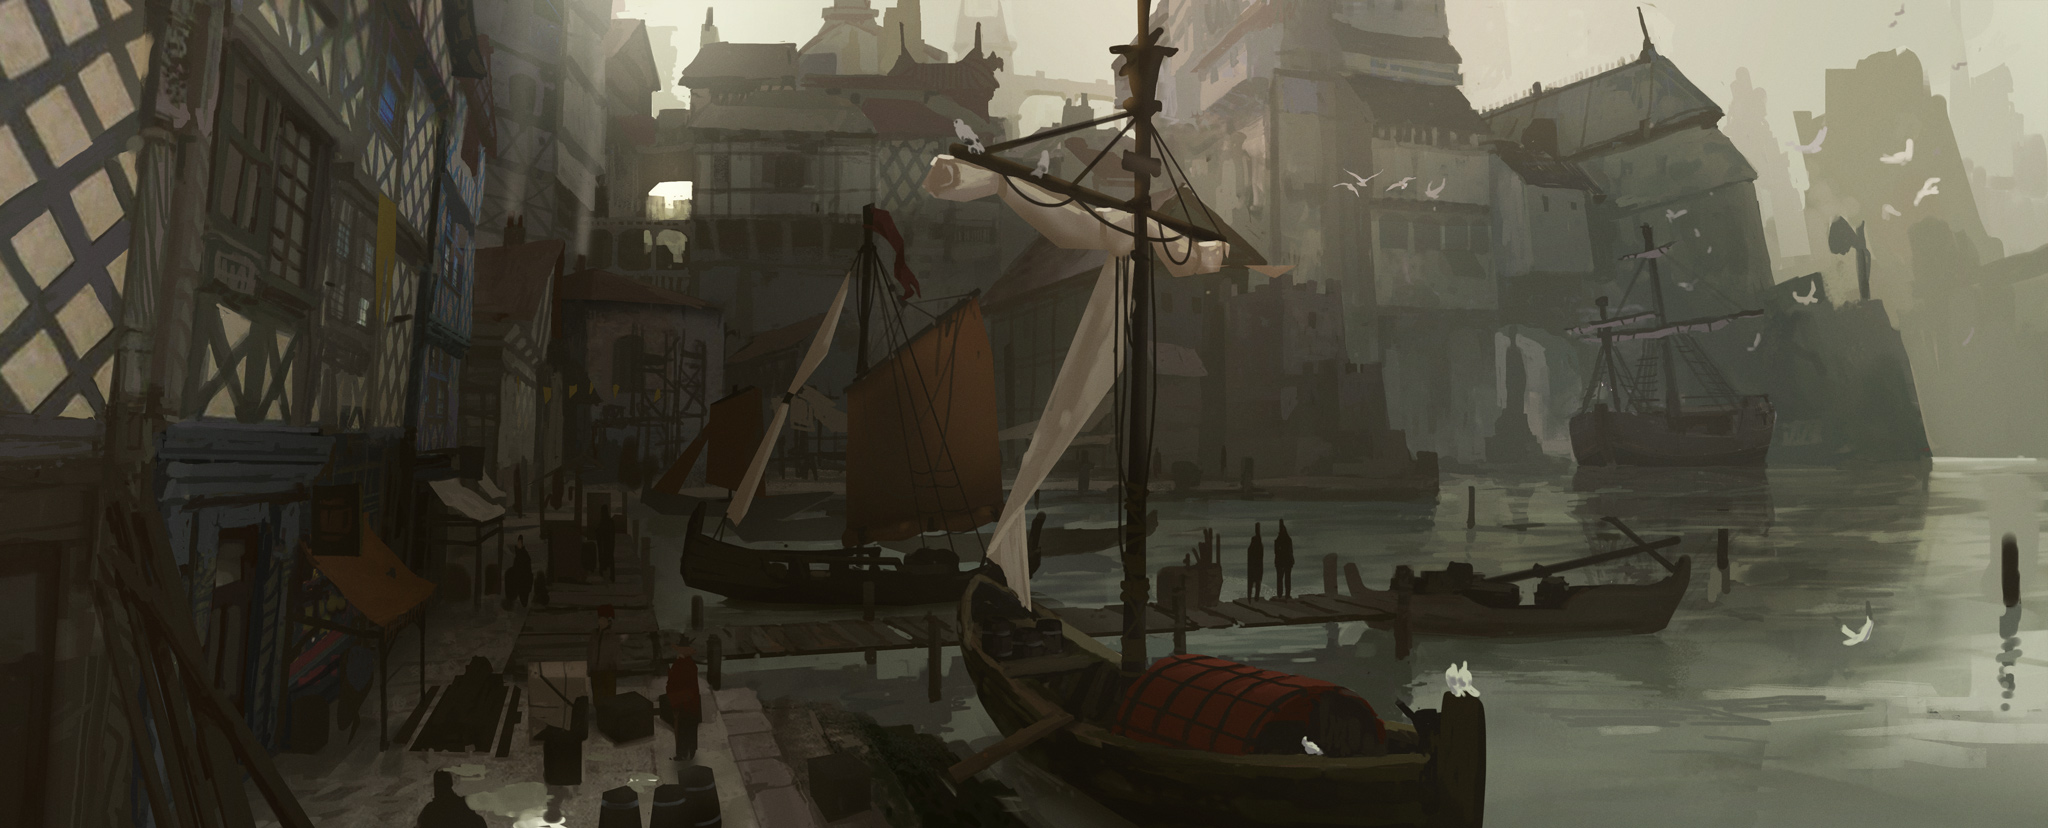
\includegraphics[width=0.95\textwidth]{valburg}

Cité-état sur la côte occidentale du continent, elle est une des principales forces commerciales de la région. Des navires de tout le monde connu y débarquent leurs marchandises : épices, tissus, ou encore matériaux de construction, presque tout peut s'échanger dans les tavernes et docks de la ville, pour qui a les contacts nécessaires et l'argent pour acheter.

Les décisions sont prises par un conseil des citoyens les plus influents de la ville, souvent parmi les plus riches. Parmi eux, un premier conseiller, ou première conseillère, est nommé afin de représenter la ville à l'étranger, et prendre les décisions quotidiennes. Aujourd'hui, \souverain dirige le conseil, depuis environ 5 ans, après une montée en puissance de sa famille depuis une trentaine d'années maintenant.

La cité en elle-même est bâtie là où elle peut contrôler une bonne partie de l'accès à la baie de Valburg. La ville possède également un large arrière-pays, très agricole et fertile. La défense de la ville est assurée par une milice bien entrainée, ainsi que par l'embauche de nombreux mercenaires en cas de conflit. La flotte, fierté de la ville, est financée par ses citoyens les plus riches, qui espèrent obtenir par là de l'influence politique. L'arsenal de la ville produit de nombreux navires utilisés tout autour du continent, mais met la priorité sur les galères et galéasses servant à la défense de la ville.

En plus de ses alentours immédiats, Valburg contrôle plusieurs comptoirs commerciaux autour du continent, qui permettent à ses navires de se ravitailler plus facilement, et de disposer de routes commerciales plus sûres.

C'est une flotte de Valburg qui, ayant entendu parler de la découverte d'un nouveau monde à l'ouest, est parti après une bonne préparation, et a fondé la colonie de \nomcolonie. Après le retour de la plupart des navires, chargés d'une lettre du nouveau gouverneur, une seconde flotte a été préparée, pour garantir à Valburg sa part des nouvelles découvertes, et des opportunités commerciales associées. Les personnages ont embarqué avec cette seconde flotte, afin de ravitailler et renforcer le nouveau comptoir.
\section{Les héritages en \nomorigine}
Les différents héritages suivants sont disponibles pour les personnages au départ de \nomorigine sans aucune restriction. D'autres peuvent être utilisés, après en avoir discuté avec le MJ.

La région à explorer étant d'un climat chaud et souvent humide, il n'est pas forcément utile de sélectionner des dons d'héritage adaptant le personnage au froid. Inversement, les adaptations aux climats chauds peuvent être plus adaptées. Ceci étant dit, faites comme vous l'entendez et voyez votre personnage, sachez uniquement que la résistance au froid devrait être moins utile que d'autres capacités.
\subsection{Humains}
Les humains sont dans la quasi-totalité des communautés de \nomorigine, et forment, de manière générale, une bonne part de la population. 

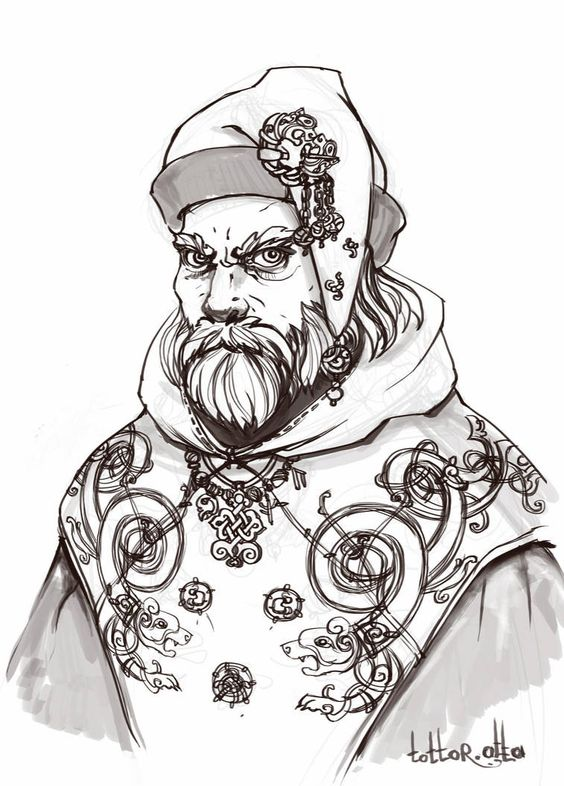
\includegraphics[width=0.49\textwidth]{humain 1}
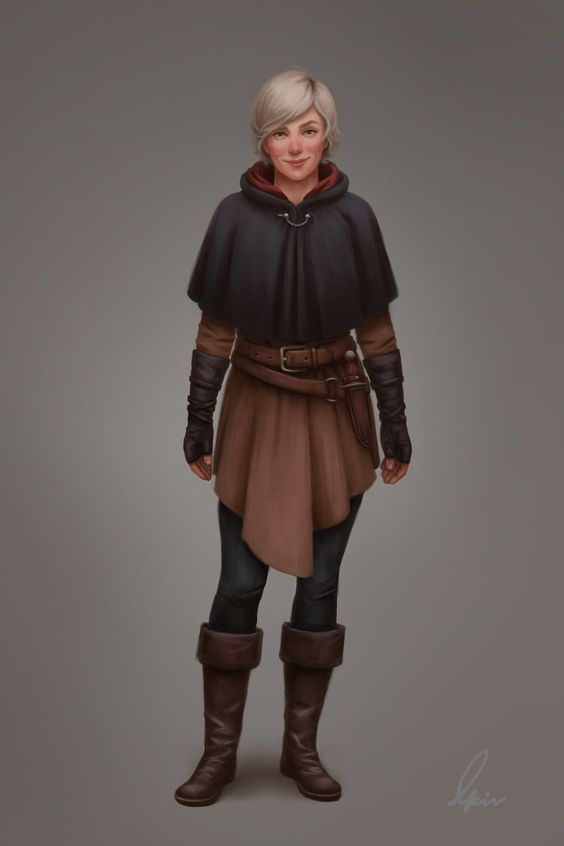
\includegraphics[width=0.49\textwidth]{humaine 2}
\subsection{Gnomes}
Les gnomes sont des créatures de petite taille, naturellement lié au royaume des fées. Ils en tirent le plus souvent une certaine extravagance et une curiosité importante. La plupart des gnomes sont naturellement de bonne humeur, une tendance qui disparait en atteignant un âge avancé.

Être un gnome, c'est souvent aller vite, voire se précipiter, changer de sujet rapidement, et de manière générale, être impatient. Pour les autres, ils peuvent paraître inconstants, imprévisibles, mais toujours de bonne humeur.

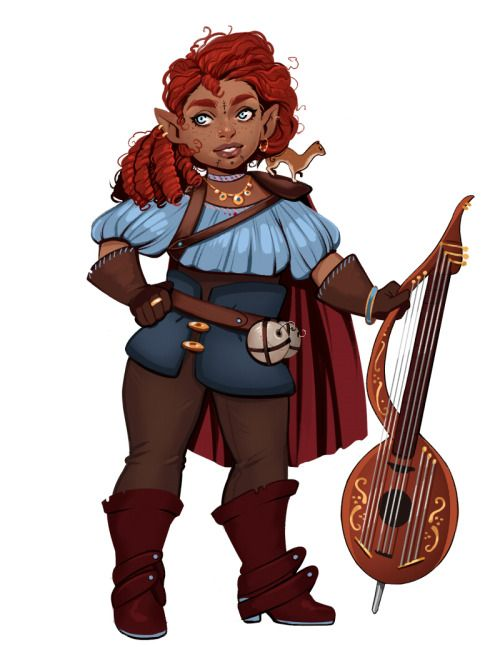
\includegraphics[width=0.49\textwidth]{gnome 1}
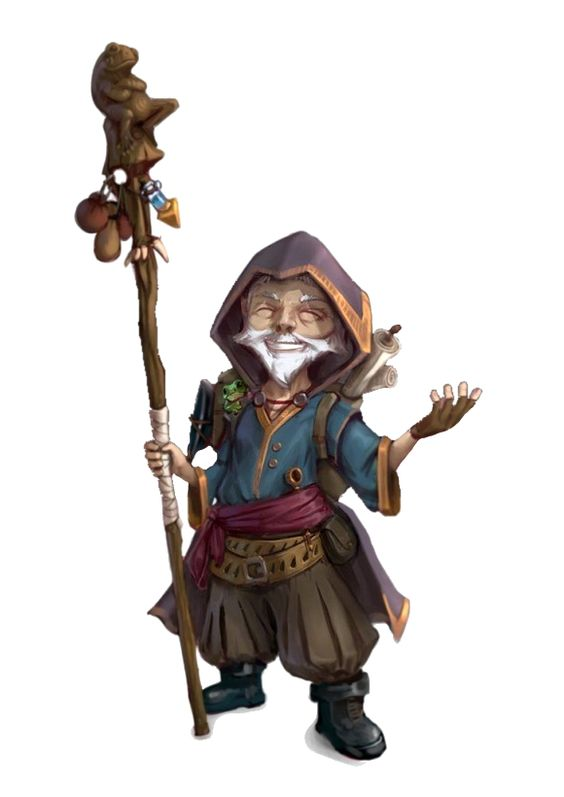
\includegraphics[width=0.49\textwidth]{gnome 2}
\subsection{Nains}
Les nains ont une petite taille, mais une forte constitution. Ils vivent essentiellement dans le nord du continent, mais des groupes spécifiques existent dans la plupart des cultures.

Les clichés sur eux impliquent généralement leur robustesse, leur patience et leur minutie, en particulier pour l'artisanat. Ils sont parfois vus comme traditionalistes et bornés, des traits qui ne sont pas partagés par tous, loin de là.

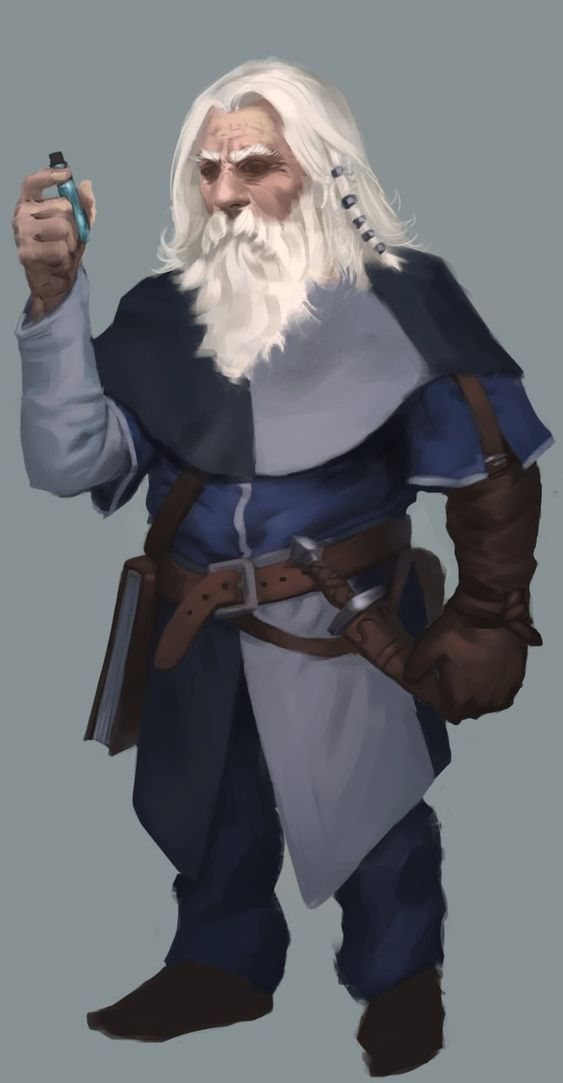
\includegraphics[width=0.49\textwidth]{nain 1}
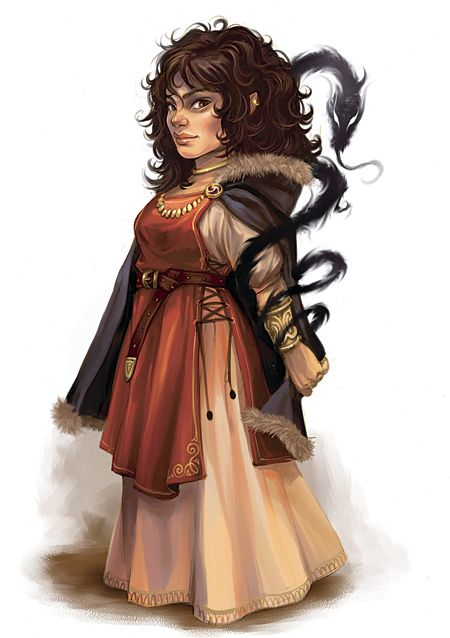
\includegraphics[width=0.49\textwidth]{naine 1}
\subsection{Elfes et demi-elfes}
Les elfes vivent longtemps, et sont généralement très adroits, voire gracieux dans leurs mouvements. Ils sont présent un peu partout sur le continent, quoiqu'un peu plus souvent vers le sud.

Leur longue durée de vie change leur point de vue sur beaucoup de situations par rapport aux autres espèces, et les clichés sur eux sont un certain détachement des affaires des autres, et une grande grâce dans leurs manières.

Les demi-elfes sont issus d'union entre des elfes et des humains, et sont stériles. Ils ont une identité complexe, sans vraiment appartenir à un monde pou l'autre. Cela peut expliquer leur grande propension à devenir aventuriers

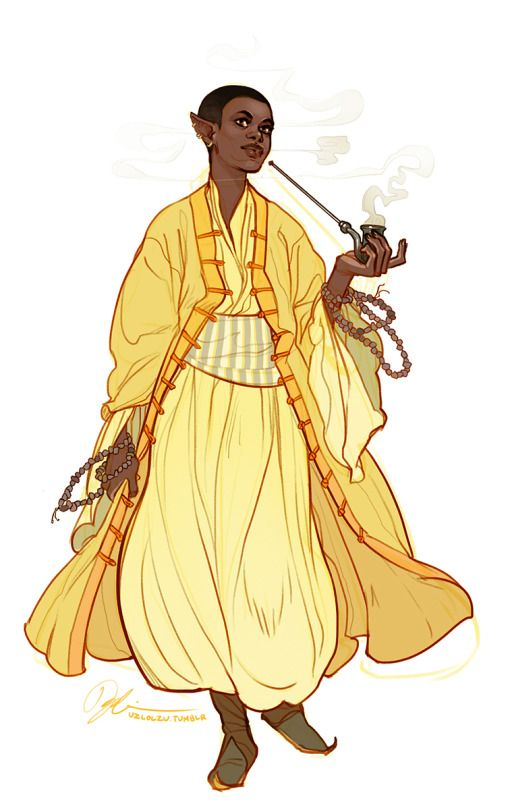
\includegraphics[width=0.49\textwidth]{elfe 1}
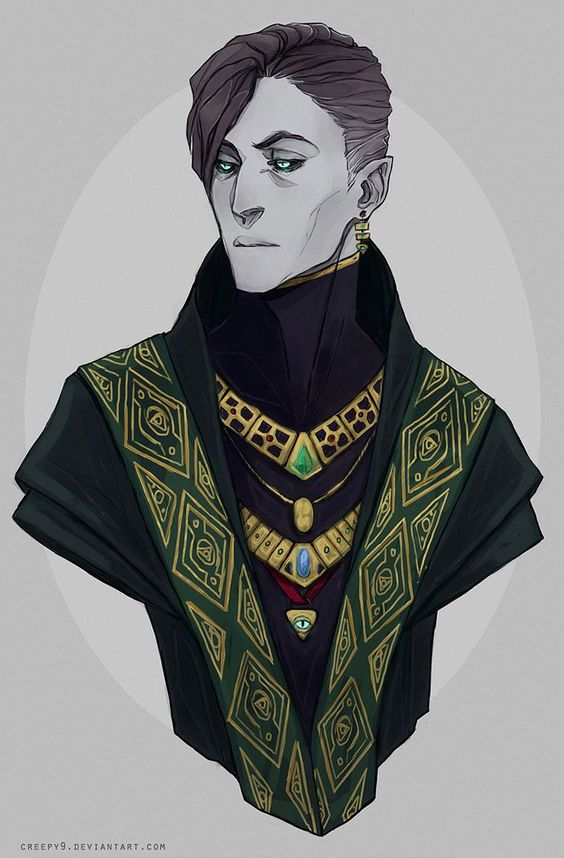
\includegraphics[width=0.49\textwidth]{elfe 2}
\subsection{Gobelins}
Les gobelins sont de petite taille, se reproduisant tant que les ressources le permettent, étant généralement tout en bas de la chaine alimentaire. On en trouve un peu partout sur le continent : dans les villes, sous terre ou dans des forêts. Une communauté de gobelins peut ne pas survivre longtemps, mais elle est rapidement remplacée par une autre.

Ils sont vus comme imprudents, parfois cruels, et souvent très actifs. Les aventuriers gobelins eux, sont souvent assez durs au mal, dynamiques et n'hésitent pas à recourir aux coups les moins loyaux.

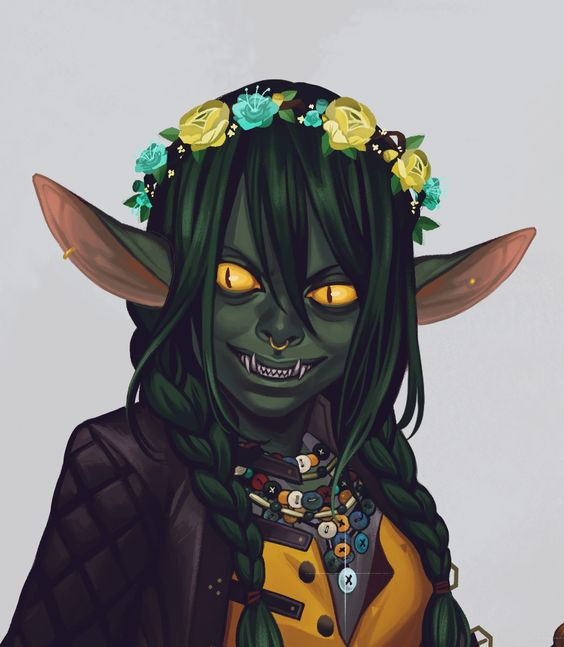
\includegraphics[width=0.49\textwidth]{gobelin 2}
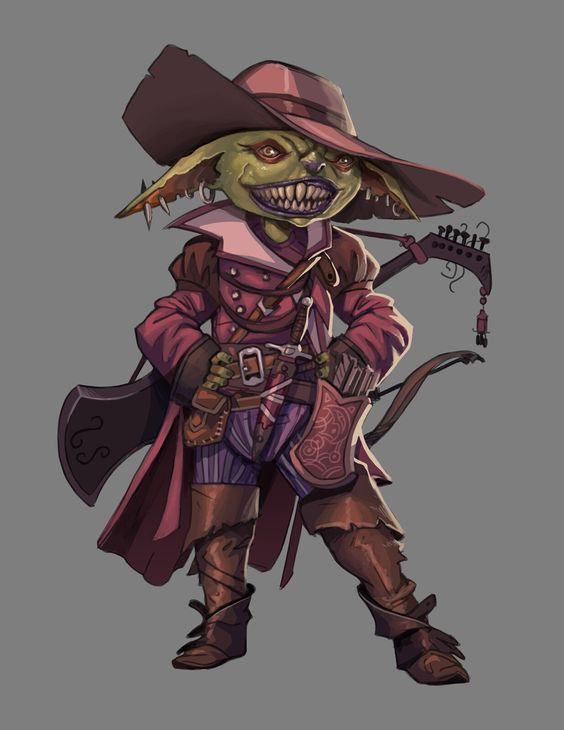
\includegraphics[width=0.49\textwidth]{gobelin 3}
\subsection{Halfelins}
Les halfelins sont également de petite taille, avec des pieds notablement poilus. Ils sont généralement très sympathiques et accueillant, et sont vus par beaucoup comme des bons vivants.

On en trouve dans une majorité du continent, mais rarement de très grandes communautés. L'aventurier archétypal est un roublard ou un alchimiste.

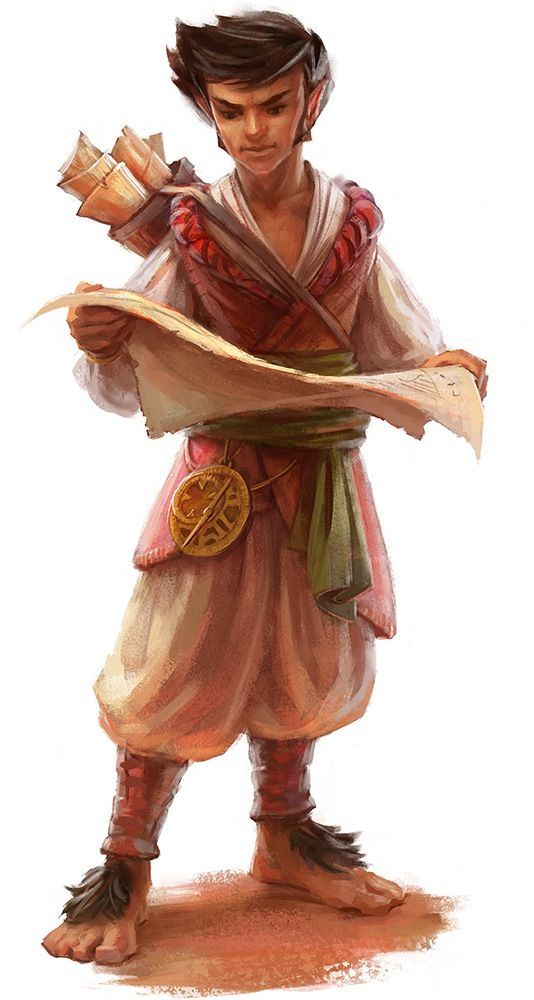
\includegraphics[width=0.49\textwidth]{halfelin 1}
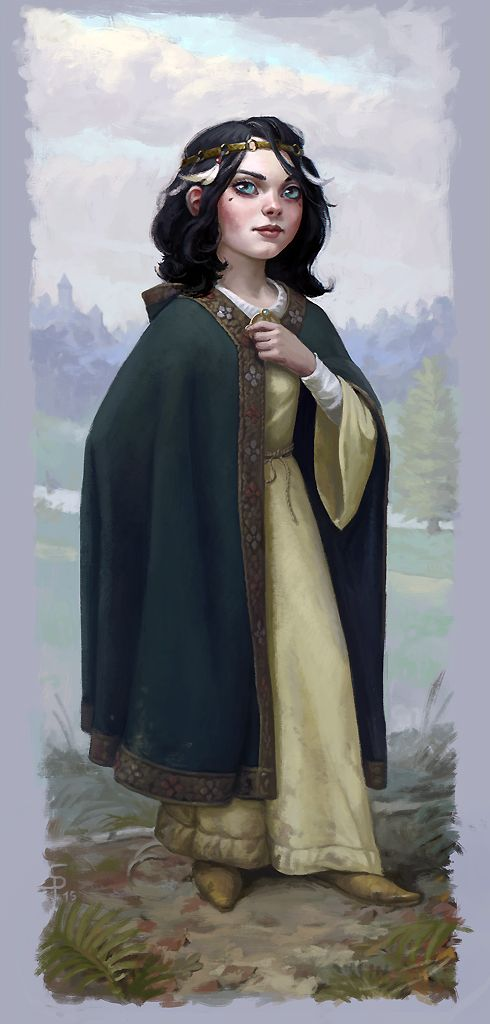
\includegraphics[width=0.49\textwidth]{halfelin 2}
\subsection{Tiefelins et Aasimar}
Les tiefelins et Aasimar portent les signes d'une ascendance infernale ou angélique respectivement, en plus de leur héritage normal. 

Les tiefelins sont rarement bien vus, étant perçus comme la preuve d'une corruption, d'un pacte passé avec des puissances maléfiques. Ils sont peu nombreux et souvent persécutés, et deviennent fréquemment des aventuriers.

Les Aasimars eux sont perçus comme une bénédiction divine, et sont traités avec beaucoup plus d'égards. Certains, énervés de cette attention, peuvent devenir aventuriers, à moins que cela ne soit pour faire quelque chose de bien directement, plutôt que de profiter de leur situation.

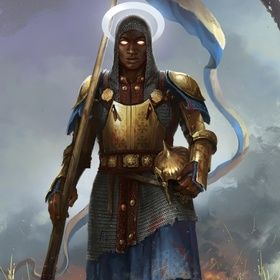
\includegraphics[width=0.49\textwidth]{aasimar 1}
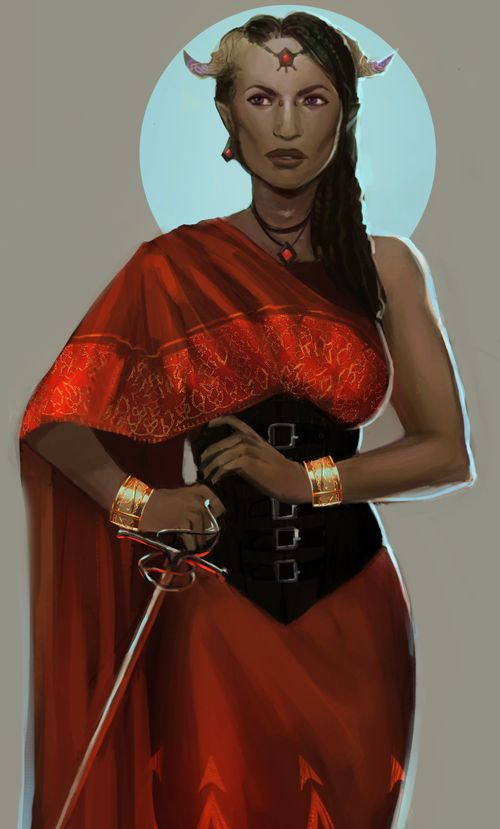
\includegraphics[width=0.49\textwidth]{tieflin 1}
\subsection{Ysoki (hommes-rats)}
Les ysoki sont une espèce d'hommes-rats, que l'on trouve le plus souvent dans les villes du continent, formant de grandes communautés très soudées. 

La majeure partie d'entre eux sont très sociaux, devenant vite inquiets tout seuls. Ils sont parfois mal perçus car vus comme proches des rats et des maladies que ceux-ci apportent.


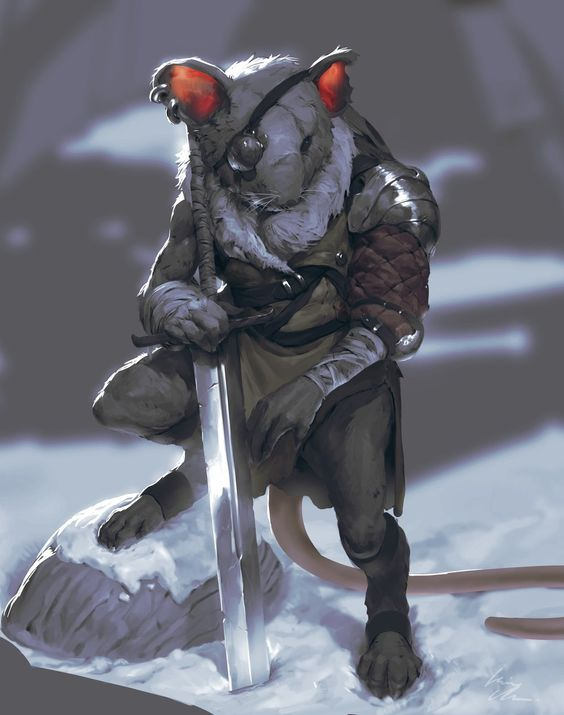
\includegraphics[width=0.49\textwidth]{ysoki 2}
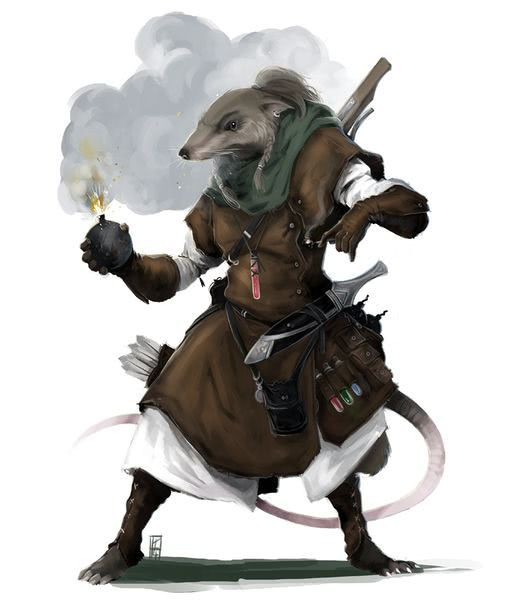
\includegraphics[width=0.49\textwidth]{ysoki 3}
\subsection{Khajit (hommes-chats)}
Les khajits sont des hommes-félins, agiles et relativement élégants. Ont les trouve surtout au sud du continent, mais quelques communautés plus adaptées au froid du nord existent également. 

Ils sont généralement plutôt individualistes, et certains leur prêtent une réputation de voleurs et de criminels potentiels. En cas de besoin, leurs griffes ne sont pas purement décorative, et peuvent faire de sérieux dégâts à un adversaire.

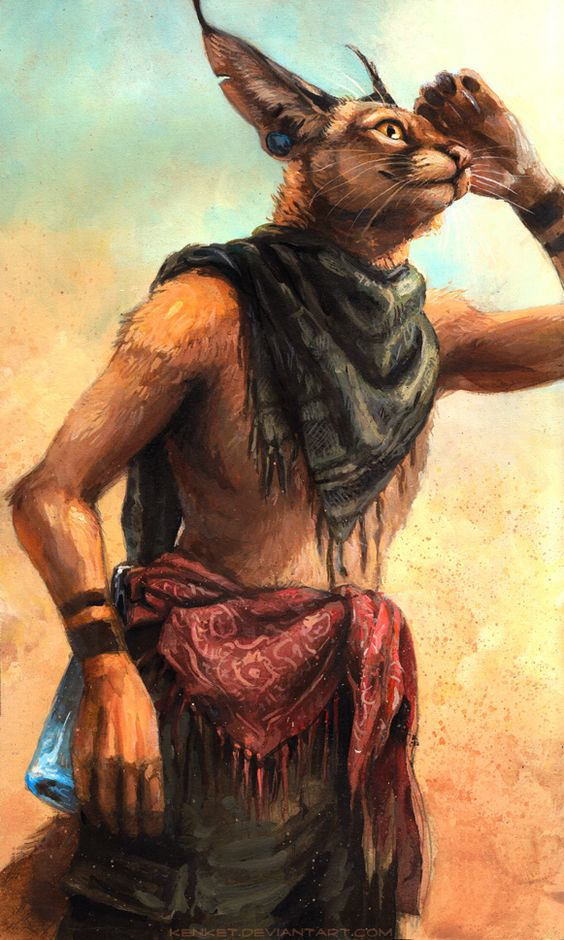
\includegraphics[width=0.49\textwidth]{khajit 2}
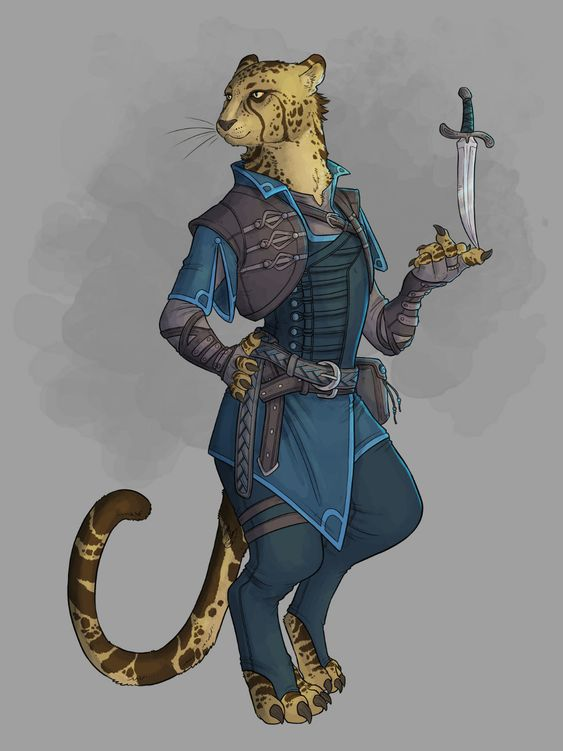
\includegraphics[width=0.49\textwidth]{khajit 3}
\subsection{kobolds}
Les kobolds sont de petites créatures reptiliennes, peut-être liées aux dragons. Comme les gobelins, ils se reproduisent très vite, pour compenser le nombre de disparitions dans leurs tribus.
La survie du groupe passe souvent avant la survie de ses membres individuels : après tout, il y en aura toujours d'autres à naître si la tribus survit.

La grande fierté de beaucoup de kobold est leur lien supposé avec les dragons : la plupart arborent des écailles aux couleurs d'une des nombreuses familles de dragons, et tous pensent en descendre, bien qu'aucun érudit n'ait pu en apporter la preuve.

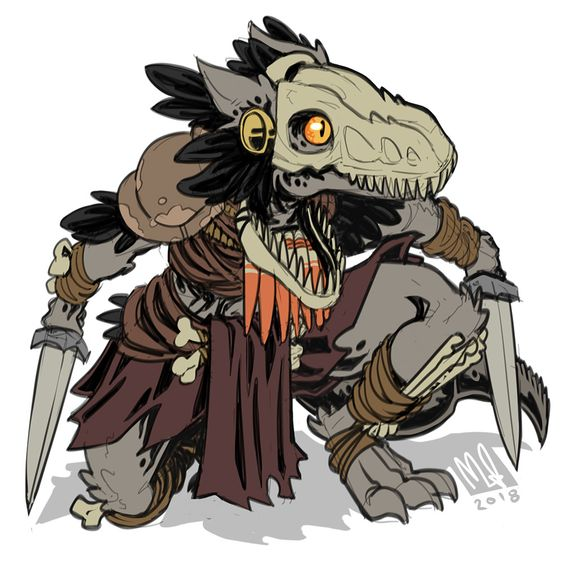
\includegraphics[width=0.49\textwidth]{kobold 2}
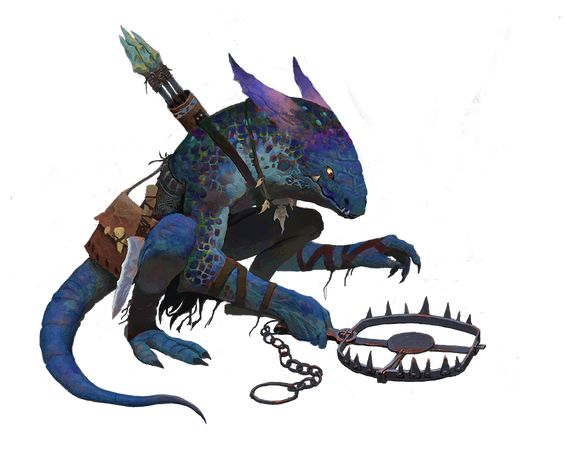
\includegraphics[width=0.49\textwidth]{kobold 3}
\subsection{Hommes-lézard}
Les hommes-lézards sont des créatures à sang-froid, bien adaptées à leur milieu naturel : des régions chaudes et souvent humides. La plupart d'entre eux sont ainsi d'excellent nageurs, et tous peuvent maintenir leur respiration pour une longue durée. Ils sont en moyenne plus grands que les humains, dépassant facilement 1m90.

Du fait de leur sang froid, les hommes-lézards peuvent être vus comme flegmatiques, ou patients, suivant les circonstances. Les traditions sont aussi souvent perçues comme importantes, au même titre que l'histoire de leur groupe (tribus, clan, nation...)

Les érudits de \nomorigine pensent que les hommes-lézards sont les héritiers d'un empire très ancien. Cela semblerait confirmer les légendes de nombreuses tribus, parfois très éloignées les unes de autres.

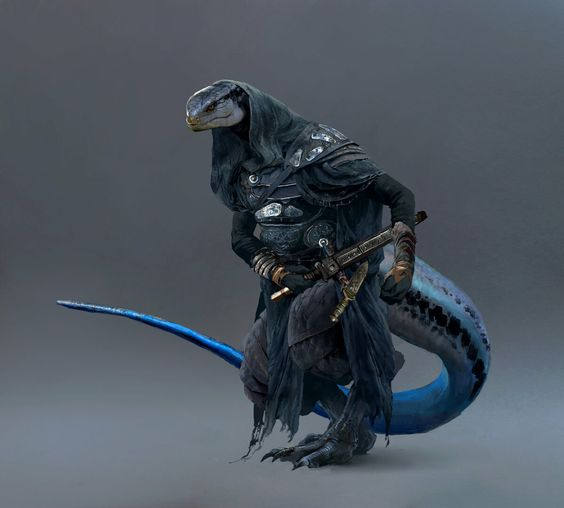
\includegraphics[width=0.49\textwidth]{lezard 1}
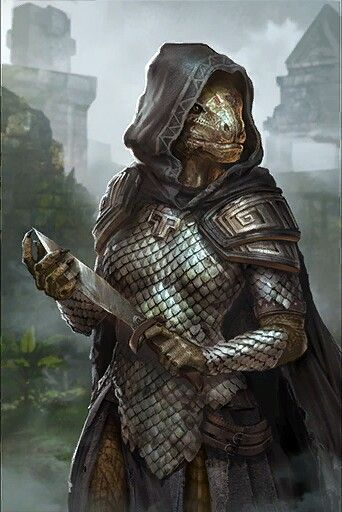
\includegraphics[width=0.49\textwidth]{lezard 2}
\subsection{tengu (hommes-oiseaux)}
Les tengu sont assez rares, mais de petites communautés existent dans les grandes villes. On parle aussi de groupes dans certaines montagnes reculées, à moins qu'ils ne viennent de terres lointaines. 

Ils sont facilement attirés par les objets brillants et les couleurs vives. Leurs gestes sont rapides et précis. Contrairement à leurs cousins les oiseaux, ils ne volent pas naturellement.

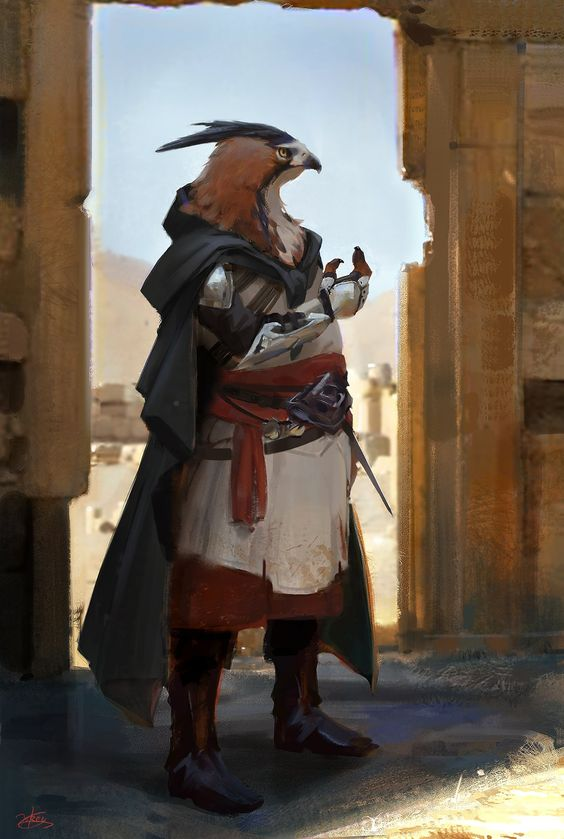
\includegraphics[width=0.49\textwidth]{tengu 1}
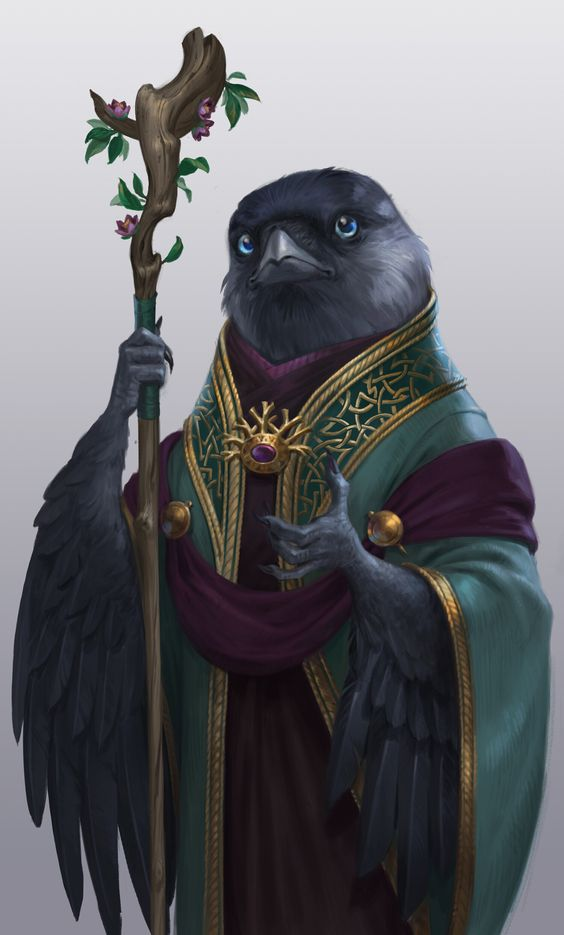
\includegraphics[width=0.49\textwidth]{tengu 2}
\subsection{Orques et demi-orques}
Relativement fréquents dans tout le continent, les orques sont une espèce généralement d'une grande taille, avec une grande puissance physique. Ils sont peu nombreux avec un statut social important.

Beaucoup s'arrêtent à leur physique et les qualifient facilement de brutes, ou de stupides. Ce n'est pas nécessairement le cas, et cette image peut les pénaliser très fréquemment.

Comme les demi-elfes, les demi-orques sont issus d'unions avec des humain(e)s, et sont souvent mal vus par les humains. les orques les acceptent plus souvent, mais beaucoup préfèrent malgré tout partir à l'aventure.

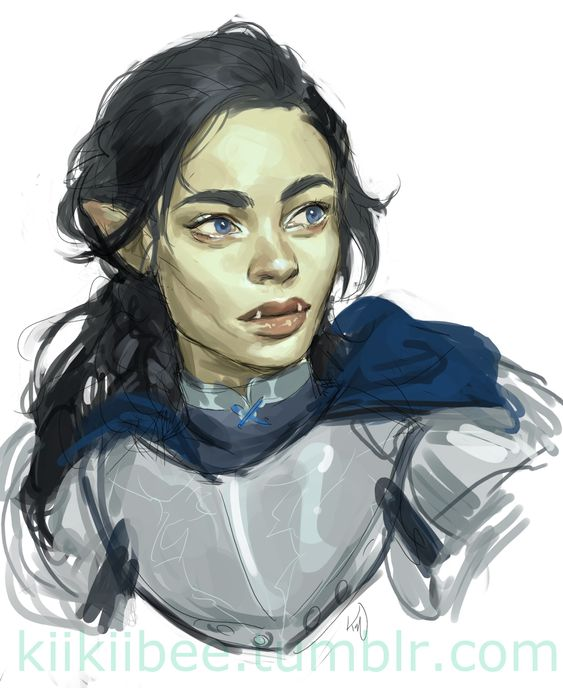
\includegraphics[width=0.49\textwidth]{orque 1}
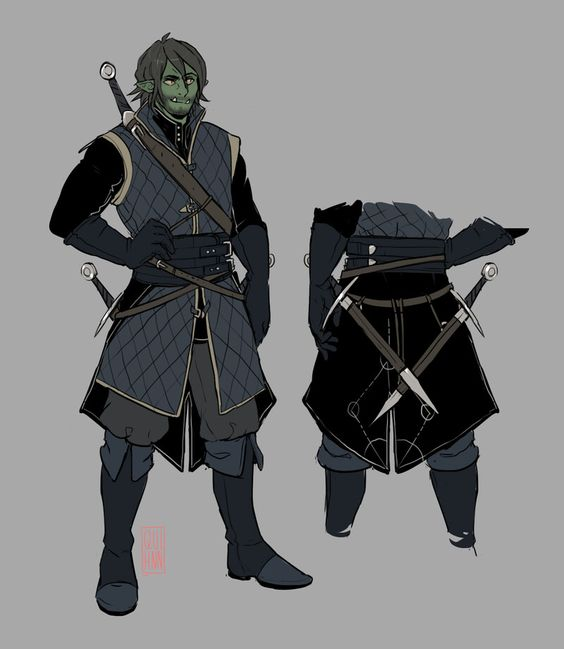
\includegraphics[width=0.49\textwidth]{orque 3}
\section{Les cultures en \nomorigine}
%noms de royaumes : Maciliens, Scannes, Harbains, Locao, Waranu
\subsection{Maciliens}
Les maciliens sont principalement présents au nord-ouest du continent, et sont le plus souvent organisés dans une société féodale : certains rois ont pu centraliser certains pouvoirs, mais la noblesse en général contrôle toujours des domaines privés.

La plupart des gens servent donc un seigneur, même si les serfs, paysans liés à une terre sans droit de la quitter, n'existent pratiquement plus. La chasse est fortement réglementée comme droit de la noblesse, mais cela n'empêche pas le braconnage. La magie est fortement surveillée par l'Eglise, bien qu'elle ne soit pas illégale.

La tenue la plus commune est composée pour les hommes d'une sous-tuniques et d'une tunique longue, ainsi que de chausses plus ou moins serrées. Ces dernières années, les manches et chausses bouffantes commencent à devenir de plus en plus à la mode.

Les aventuriers Maciliens sont souvent équipés avec du matériel de multiples origines, au vu du prix d'un matériel neuf, et sont confondus avec la profession de mercenaires.

Inspirations : The witcher (royaumes du nord), Europe nord-ouest XVème siècle

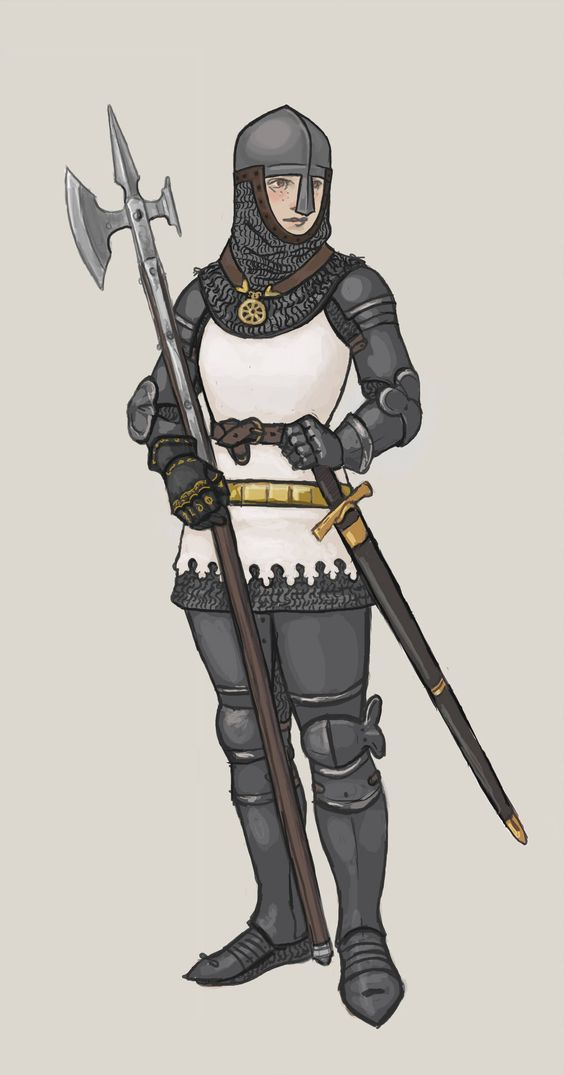
\includegraphics[width=0.49\textwidth]{humaine 1}
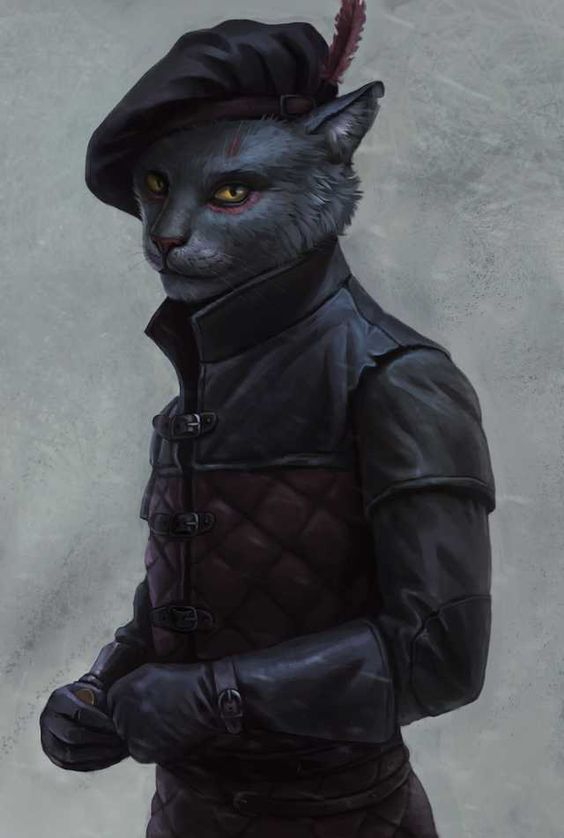
\includegraphics[width=0.49\textwidth]{khajit 1}
\subsection{Scannes}
L'empire Scannien contrôle une bonne part du centre et de l'est du continent, et présente une économie florissante, à défaut d'avoir une situation politique très stable.

Le service au sein de l'armée impériale reste le plus court chemin pour travailler dans les administrations des provinces, et la citoyenneté obtenue est une motivation pour beaucoup de sujets de l'empire.

Plus qu'une culture indépendante, c'est aussi un melting pot dans lequel de nombreuses cultures de la région se retrouvent après leur conquête. Les vêtements sont donc extrêmement variés suivant le climat régional, avec souvent des couleurs chatoyantes et pour ceux qui peuvent se le permettre, des tissus riches, comme la soie.

Inspirations : empire byzantin, morrowind (dunmers)

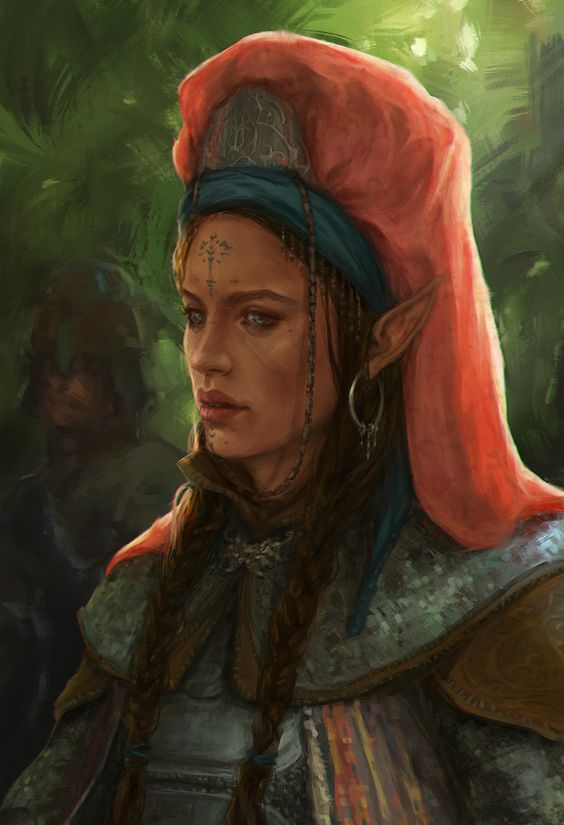
\includegraphics[width=0.49\textwidth]{elfe 3}
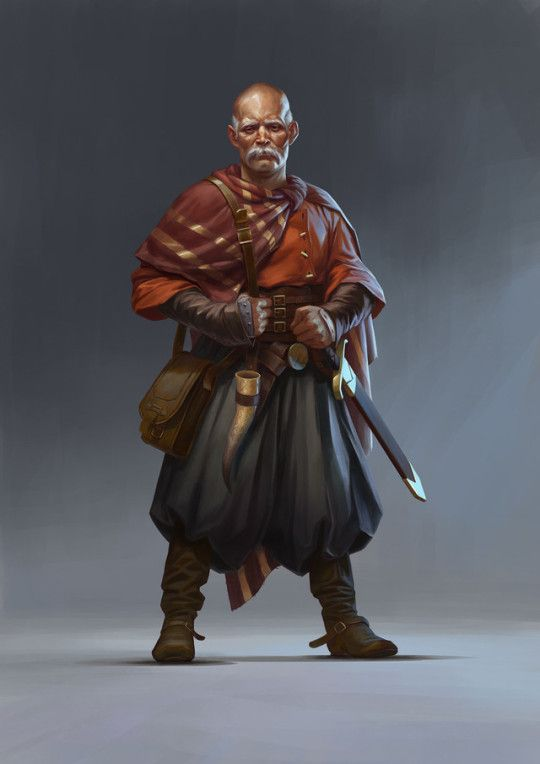
\includegraphics[width=0.49\textwidth]{humain 3}
\subsection{Harbains}
Les harbains forment un ensemble de royaumes et de cité-états au sud des royaumes maciliens, et sont réputés pour se battre plus fréquemment entre eux que face à d'autres cultures. Valburg est de culture majoritairement Harbaine.


Les tenues à la mode impliquent des sections bouffantes, et si possible percées pour révéler une couche inférieure contrastante. A cette mode plutôt urbaine s'ajoute des tenues plus traditionnelles très chatoyantes et brodées dans les campagnes.

Les aventuriers sont nombreux dans ces régions souvent en conflit, et où la politique joue un grand rôle en ville. Il s'agit peu souvent de chasser des bêtes, et beaucoup plus d'affronter des hommes.

inspirations : Italie XV-XVIème siècle, Europe début renaissance

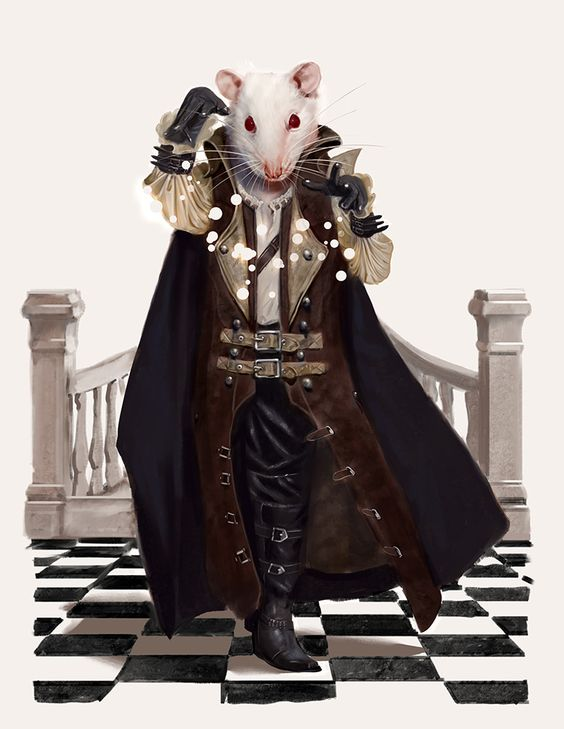
\includegraphics[width=0.49\textwidth]{ysoki 1}
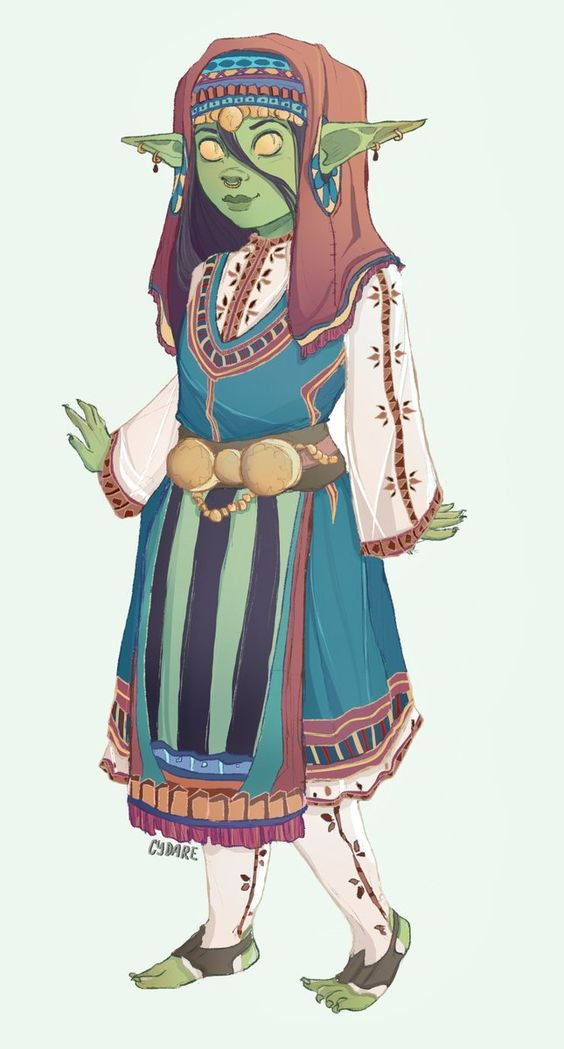
\includegraphics[width=0.49\textwidth]{gobelin 1}
\subsection{Sonons}
Les sonons étaient il y a quelques siècles la terreur de la totalité du nord de \nomorigine, pillant à volonté les villes et monastères, et imposant leur loi sur les royaumes de environs. La constitution de l'empire Scanne les a repoussé vers le nord, de même que des défenses plus importantes dans d'autres lieux. Du fait de leurs expéditionss, on trouve des Sonons dans la totalité de la moitié nord du continent.

Leurs tenues sont adaptées aux plaines glacées du nord, ainsi qu'à la navigation. Elles comportent donc plusieurs couches, souvent avec de la laine et/ou de la fourrure. 

Politiquement, il s'agit le plus souvent de petits royaumes isolés, généralement constitués autour d'une ville principale. Le fait de posséder des terres arables est un signe de statut important, et garantit une grande maisonnée ainsi qu'un bon équipement militaire.

Les aventuriers sont très nombreux à venir de ces terres, où le pillage est une sorte d'ancienne tradition, tout comme le fait de chercher la gloire en tuant des créatures de grande taille.

inspirations : russie médiévale, scandinavie, mongolie

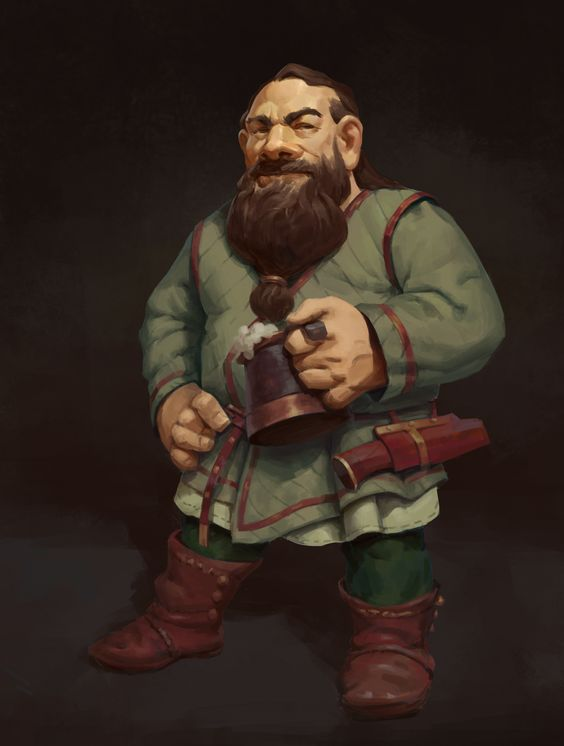
\includegraphics[width=0.49\textwidth]{nain 2}
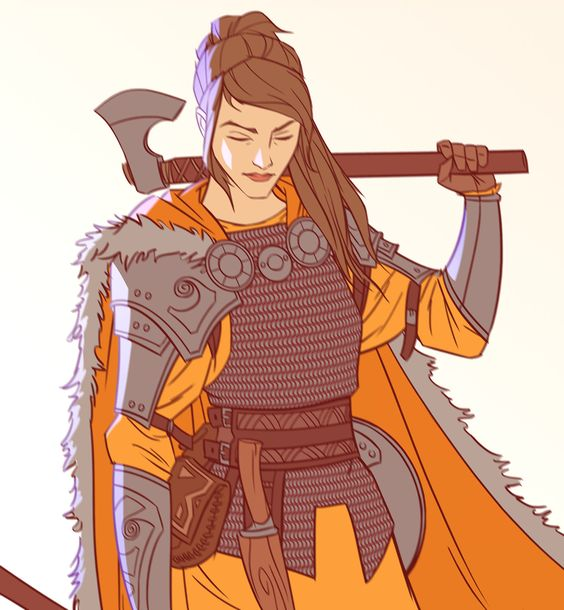
\includegraphics[width=0.49\textwidth]{humaine 3}
\subsection{Locao}
Les locaos vivent autour et dans une région au centre du continent généralement aride, à l'exception de quelques fleuves fertiles. Quelques villes ont été construites le long de ceux-ci, et sont d'important centres de commerce, mais sinon, beaucoup de gens vivent dans les terres arides, ou sont nomades, parcourant le Grand Désert pour y transporter marchandises et étrangers.

Les tenues extérieures sont généralement très couvrantes et amples, sauf pour les habitants à sang-froid ou qui résistent aux températures élevées. 

Les sociétés sont généralement très organisées, et hiérarchisées chacun ayant un rôle spécifique à accomplir. cela est moins vrai dans les villes, mais dans le désert, celui qui ne rempli pas son rôle est un paria, abandonné par les siens.

Inspiration : perse, égypte antique, califats arabes, Dragon age (Qunari)

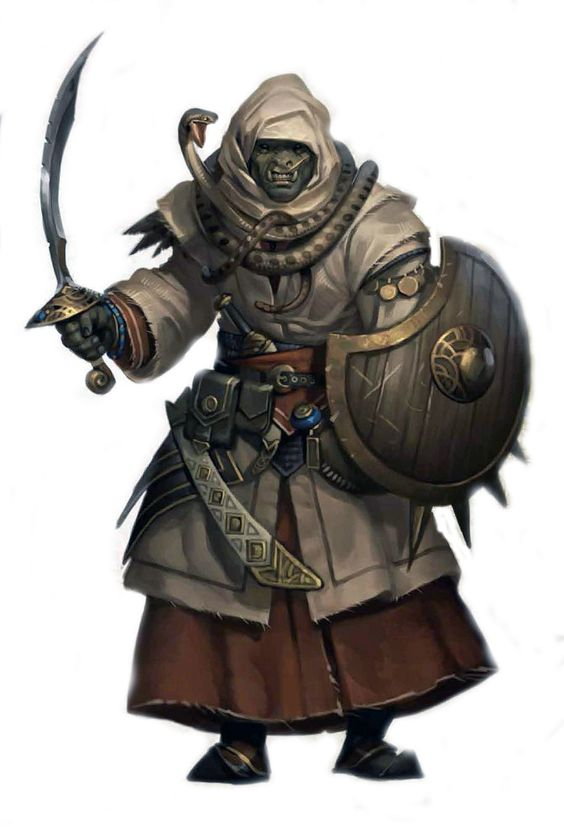
\includegraphics[width=0.49\textwidth]{orque 2}
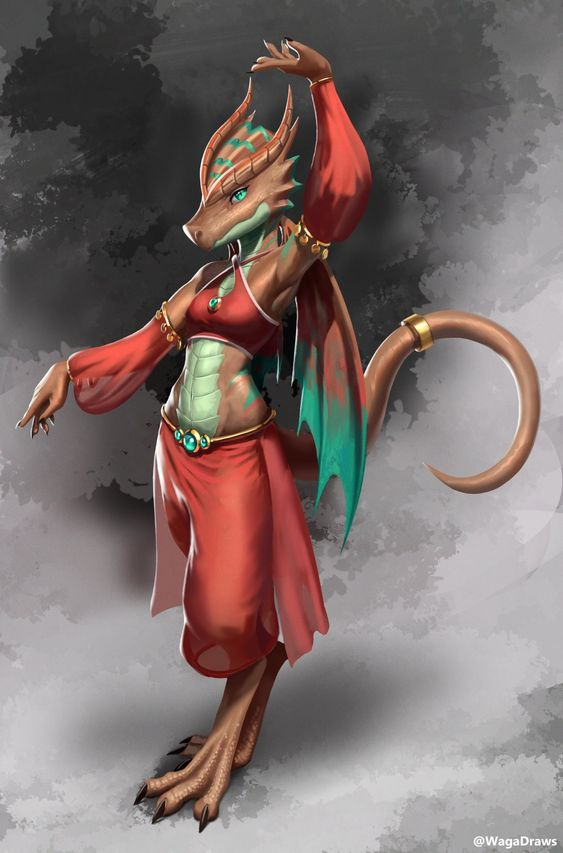
\includegraphics[width=0.49\textwidth]{kobold 1}
\subsection{Waranu}
Les waranu occupent une partie du sud-ouest du continent, un empire immense regroupant en réalité plusieurs cultures distinctes. L'empire a eu plusieurs périodes d'expansions et de diminution, suivant sa stabilité. La dernière grande réduction a eu lieu au siècle dernier, quand les mages de l'Urundo (un conseil de mages qui dirigeaient l'empire) ont été tué suite à l'insurrection de la plupart des églises

Les grandes villes sont de haut lieux du savoir, parfois même trop, l'histoire de l'Urundo et ses abus étant encore frais dans les mémoires. Dans tous les cas, savants et lettrés du monde entiers viennent dans les villes Waranu pour y chercher des connaissances.

les modes varient énormément d'une province à l'autre, le point commun étant les riches bijoux, souvent en or, que tous ceux qui le peuvent arborent.

Inspiration : empire éthiopien, Dragon Age (Tevinter)

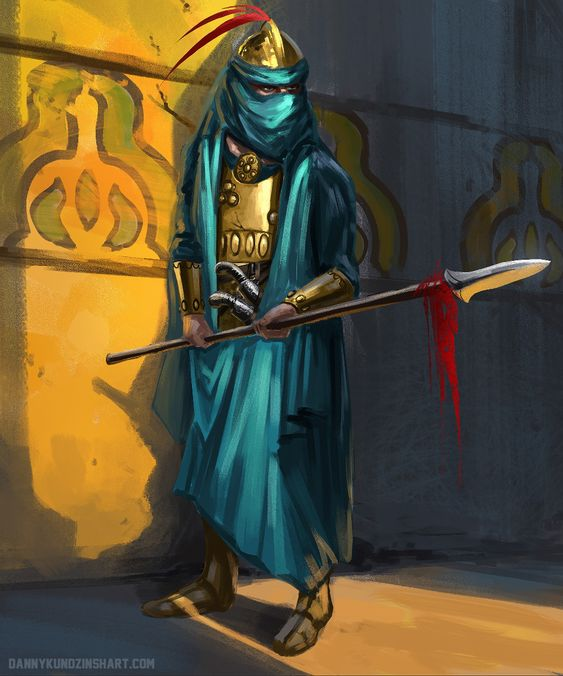
\includegraphics[width=0.49\textwidth]{humain 5}
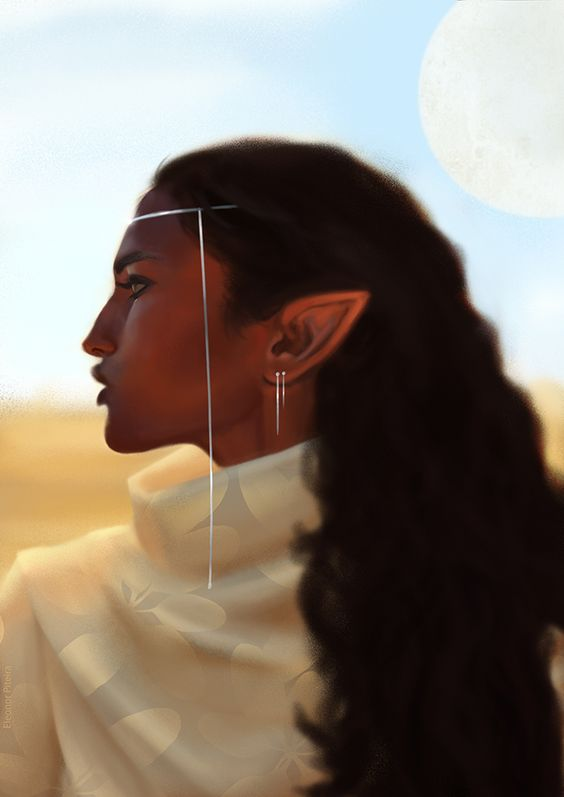
\includegraphics[width=0.49\textwidth]{elfe 4}

\section{La religion}
De nombreux dieux sont vénérés en \nomorigine, les plus importants et répandus sont décris ci-dessous. Il est tout à fait possible de vénérer une autre divinité, après discussion de celle-ci avec le MJ.

L'édit d'une divinité correspond aux règles les plus importantes suivies par ses fidèles, et en particulier par son clergé, les anathèmes sont à l'inverse, les actions interdites, sous peine d'attirer la défaveur de la divinité. Les autres éléments décris sont en rapport avec les règles de religion, principalement pour les clercs et champions.
\subsection{Dynris, la tisseuse du destin}
Déesse des rêves et gardienne des âmes des morts, qu'elle permet parfois de traverser le voile pour discuter en rêves. Elle tisse les fils du destin, patiemment : au bout du compte, toutes les âmes viendront dans son domaine onirique. Elle est représentée sous les traits d'une jeune femme, tissant sous la lumière de la lune. Le symbole le plus commun de son Eglise est un croissant de lune, et la plupart de leurs cérémonies ont lieu une fois la nuit tombée, quand la déesse parcourt les âmes des hommes. Elle est parfois représentée comme la muse des artistes, inspirant ceux-ci dans leur sommeil. Ses serviteurs offrent un soutien moral à ceux qui sont en deuil, et fournissent autant que possible un soutien aux artistes.

C'est une déesse solitaire, et plutôt bienveillante, malgré son rôle. La chose causant son courroux est l'animation de morts-vivants, en particulier les morts-vivants ayant conservé leurs âmes : ce sont des abominations qui doivent être anéantis.
\paragraph{Édit} Rassurez et inspirez ceux qui vous entourent, faites leur profiter de la vie.
\paragraph{Anathème}S'associer à un mort-vivant conscient, Lancer un sort comme Cauchemar.
\paragraph{Alignement des serviteurs} Neutre, Neutre Bon, Chaotique Bon
\paragraph{Arme favorite } Coutille
\paragraph{Canalisation} Soin
\paragraph{Compétence}médecine ou performance
\paragraph{Sorts de clercs}Couleurs dansantes (niveau 1), message onirique (niveau 3), assassin spectral (niveau 4)
\paragraph{Domaines }Rêves, mort, destin, lune
\subsection{Khimros, aussi appelé Hilous dans le sud du continent}
Le bâtisseur et protecteur des cités. Il inspire tous ceux qui construisent de leur mains : artisans et maçons, mais aussi ceux qui protègent la civilisation et l'ordre. Il a un temple dans toute grande ville, et ses serviteurs essaient souvent d'y maintenir l'ordre, ainsi que sur les routes majeures. Ils encouragent également la création sous toute ses formes, en particulier l'artisanat : forge, maçonnerie, tissage....

Il est représenté sous les traits d'un homme d'âge mûr, dans une tenue simple et pratique. Il est marié à Itia, l'accueillant à chaque retour de ses voyages dans leur domaine, toujours plus beau et mieux pensé. Il tient souvent son marteau, tant un outil pour bâtir qu'une arme pour défendre ses créations. Ce marteau est le symbole de son église pratiquement partout.
\paragraph{Édit} Maintenez l'ordre et la sécurité dans les royaumes mortels, et participez à l'avancée des civilisations.
\paragraph{Anathème} Détruire un objet d'art ou d'architecture important, créer un conflit.
\paragraph{Alignement des serviteurs} Loyal Bon, Loyal Neutre, Neutre Bon.
\paragraph{Arme favorite } marteau de guerre
\paragraph{Canalisation} Soin
\paragraph{Compétence} Artisanat
\paragraph{Sorts de clercs} objet illusoire (niveau 1), création (niveau 4), manoir magnifique (niveau 7)
\paragraph{Domaines }Cités, création, famille, richesse.
\subsection{Yor, Kuvasis ou Mazotl, la bête}
C'est le dieu du chaos, de la destruction et de la douleur. Il apprécie de voir les civilisations s'effondrer, les villes être piller, et les connaissances se perdre. 

Ses serviteurs essaient de miner les lois, de rendre moins sûres les routes et de détruire des objets ou connaissances importantes pour satisfaire leur divinité, en espérant être récompensés pour cela. Ils sont peu nombreux, et leur culte est très souvent illégal, donc dispersé. Ils n'ont pas de symbole très défini, souvent un œil de couleur noire ou rouge.

Frère cadet de Khimros, il en est jaloux, et fait tout pour mettre à bas ses créations. Il s'entend peu avec les autres dieux, ce qui lui va bien : il compte bien apporter un jour la fin des temps, et gagner face à eux tous !
\paragraph{Édit}Brisez l'emprise de l'ordre et de la loi sur le monde, détruisez les villes et ramenez le monde à un état plus primitif.
\paragraph{Anathème} Fournir un soutien à ceux qui souffrent, ou une protection à ceux qui en ont besoin.
\paragraph{Alignement des serviteurs} Chaotique mauvais, Neutre Mauvais, Chaotique Neutre
\paragraph{Arme favorite }Serpe
\paragraph{Canalisation} Blessure
\paragraph{Compétence}Subterfuge
\paragraph{Sorts de clercs}crocs magiques (niveau 1), agrandissement (niveau 2), désintégration (niveau 6)
\paragraph{Domaines }Ténèbres, cauchemar, douleur, destruction
\subsection{Uton, l'ombre}
Divinité des secrets, de la vérité, et de la non-mort, son culte est rarement public, à l'exception de son rôle dans la justice : la découverte de la vérité. Étonnamment, il est aussi prié par certains criminels, pour qu'il protège leurs ruses.

Au delà de son conflit avec Dynris, pour obtenir les secrets que la mort cache, il est vu comme un mal nécessaire par d'autres divinités, comme Khimros, ou un allié par Ione, qui apprécie sa recherche de vérité.

Il n'est jamais représenté directement, seule une silhouette de lui est esquissée, le plus souvent de manière éphémère : une marque au charbon ou à la craie est privilégiée à une gravure. Ses temples sont nomades, ses fidèles se retrouvant dans des lieux perdus ou peu empruntés, et en changeant régulièrement.
\paragraph{Édit} Améliorez votre compréhension du monde, propagez la vérité, travaillez en secret.
\paragraph{Anathème} Transformer une situation pacifique en conflit ouvert, détruire une importante vérité, détruire un mort-vivant conscient.
\paragraph{Alignement des serviteurs} Chaotique neutre, Neutre, loyal Neutre.
\paragraph{Arme favorite }kukri
\paragraph{Canalisation} Soin ou Blessure
\paragraph{Compétence} discrétion
\paragraph{Sorts de clercs}déguisement (niveau 1), invisibilité (niveau 2), assassin spectral (niveau 4)
\paragraph{Domaines }Secrets, Ruse, Non-mort, Vérité
\subsection{Inmes, le dernier-né}
Divinité majeure la plus récente à être née, il était autrefois un mortel à l'ambition sans limite. Par ses paroles ou par ses armes, il mis au pas une grande part du continent, créant l'empire d'Oraxos. A sa mort, ses successeurs en firent un culte à la gloire de l'empire, jusqu'à son effondrement, tant et si bien qu'il pu quitter le domaine de Dymris, pour prendre sa place parmi les immortels, ayant accompli son ultime ambition. Pour les mortels, il est l'incarnation de l'ambition, des passions, de la recherche de perfection, mais aussi le premier tyran à avoir foulé les royaumes mortels.

Le symbole de son église, depuis sa fondation, est l'aigle impérial, ailes déployées et jugeant ceux qui se trouve devant lui. Il est représenté tel que les statues impériales le représentaient : un homme grand, fort, à la riche tenue. Il est souvent représenté avec un fouet à la main.
\paragraph{Édit} Soyez supérieurs à vos serviteurs, et respectueux de vos supérieurs, respectez votre parole.
\paragraph{Anathème} Briser un contrat, montrer de la pitié envers un ennemi, libérer un esclave. 
\paragraph{Alignement des serviteurs}Neutre Mauvais, Loyal Neutre, Loyal Mauvais
\paragraph{Arme favorite } Fouet
\paragraph{Canalisation} blessure
\paragraph{Compétence}intimidation
\paragraph{Sorts de clercs}charme (niveau 1), suggestion (niveau 4), tromperie (niveau 6)
\paragraph{Domaines }passion, perfection, tyrannie et ambition
\subsection{Urasil ou Byemer, l'implacable}
Dieu des combattants, il est celui qui prête sa volonté indomptable aux mortels, et leur a amené le feu dans ses mains.

Il est vénéré par les guerriers de tout le continent pour qu'ils vainquent leurs ennemis, ou survivent à la journée pour combattre un autre jour. Ses temples contiennent tous un feu éternel, et chaque fidèle est tenu d'apporter du combustible pour le maintenir vivace.

C'est un dieu exigeant, presque autant envers les autres qu'en vers lui-même. Il est représenté sous les traits d'un soldat, couturé de cicatrice, ou d'un vieillard, marqué par les épreuves de la vie. La flamme éternelle est le symbole de son église.
\paragraph{Édit} Atteindre la victoire en combat équitable, dépasser ses limites, entretenez le moral de ceux qui sont autour de vous.
\paragraph{Anathème} Laisser le feu sacré s'éteindre, vaincre par traitrise, négocier une solution pacifique à un problème militaire.
\paragraph{Alignement des serviteurs} Chaotique neutre, Neutre, Chaotique Bon.
\paragraph{Arme favorite } épée à deux mains
\paragraph{Canalisation} blessure ou soin
\paragraph{Compétence}athlétisme
\paragraph{Sorts de clercs} coup au but (niveau 1), agrandissement (niveau 2), tempête d'armes (niveau 4)
\paragraph{Domaines }Zèle, chance, force feu
\subsection{Bragta, la nourricière}
Déesse-mère, protectrice des cultures et de la nature, et éternelle bienveillante envers les mortels.

Elle est représentée sous les traits d'une femme robuste, et souvent avec des outils de fermiers, dont le fléau. Ses serviteurs sont très nombreux dans les campagnes, où ils aident les paysans à subsister, tout en maintenant l'équilibre avec la nature. Beaucoup sont ascétiques, se passant le plus souvent de viande.

Le symbole de son église est un boisseau de blé, que l'on trouve au fronton de chacun de ses temples.
\paragraph{Édit} Protégez la nature et les innocents, assurez vous que tous aient de quoi se nourrir. Fondez une famille.
\paragraph{Anathème} Tuer une créature innocente, affamer quelqu'un, abandonner votre foyer en temps de besoin, placer vos besoins avant ceux de votre communauté.
\paragraph{Alignement des serviteurs} Neutre Bon, Chaotique Bon, Chaotique Neutre
\paragraph{Arme favorite } Fléau
\paragraph{Canalisation} Soin
\paragraph{Compétence} Nature
\paragraph{Sorts de clercs} 
\paragraph{Domaines }Coup de vent (niveau 1), éclair (niveau 3), contrôle des eaux (niveau 5)
\subsection{Ione, déesse des profondeurs}
La déesse de la mer, mais aussi de la connaissance et de la magie. Son domaine sous-marin est réputé être la plus grande bibliothèque des plans. Elle est vénérée tant par les marins que par les mages, pour ses différents aspects.

Elle est représentée sous de nombreux traits : une magicienne expérimentée, une sirène dans son domaine, ou encore une jeune fille de pêcheur, un panier plein des fruits de la mer.

Elle est souvent vue comme capricieuse, même par ses serviteurs, qui apprennent à endurer les mauvais moments pour profiter des bons. Les voyageurs la prient pour améliorer son humeur sur leur route. Son église n'a pas de symbole défini.
\paragraph{Édit} Protégez la connaissance, acceptez les changements, contrôlez-vous
\paragraph{Anathème} Détruire une connaissance ou une créature magique importante, rester trop longtemps au même endroit
\paragraph{Alignement des serviteurs} Loyal Neutre, Neutre, Chaotique Neutre
\paragraph{Arme favorite }Trident
\paragraph{Canalisation} Soin ou Blessure
\paragraph{Compétence} Arcane
\paragraph{Sorts de clercs} lien mental (niveau 1), léviter (niveau 3), contrôle des eaux (niveau 5)
\paragraph{Domaines } Eau connaissances, voyages, magie
\subsection{Eris, protectrice des mortels}
Eris est la déesse de la lumière, des airs et du soleil. Ses dons servent à protéger les mortels depuis l'aube des temps.

Son église s'intéresse à tous, en particulier ceux qui ne peuvent se défendre : les pauvres, les malades, ou simplement ceux qui sont attaqués par des créatures.

Elle est présentée sous les traits d'une femme en armure, avec des ailes angéliques, portant assistance à ceux qui en ont besoin.
\paragraph{Édit} Protégez ceux dans le besoin, affrontez les tyrans, luttez contre l'injustice.
\paragraph{Anathème} Nier à une créature la possibilité de se rependre de ses crimes, tolérer les diables et démons, créer une zone de ténèbres.
\paragraph{Alignement des serviteurs} Chaotique Bon, Neutre Bon, Chaotique Neutre
\paragraph{Arme favorite }Lance (spear en anglais)
\paragraph{Canalisation} Soin
\paragraph{Compétence} Médecine ou société
\paragraph{Sorts de clercs}coup au but (niveau 1), voire l'invisible (niveau 2), bouclier de feu (niveau 4)
\paragraph{Domaines }Air, soleil, protection, bonté
\subsection{Itia déesse des messagers}
La messagère des dieux, celle qui amène les messages divins sur terre. De part le pacte conclu entre les immortels, elle est la seule à pouvoir intervenir directement auprès des mortels, et se doit de rester neutre vis-à-vis des autres dieux, ce qui n'a pas manqué de causer des conflits : avec Yor et Urasil pour leurs interventions et son mari Khimros, qui lui reproche parfois sa neutralité.

Elle est représentée sous les traits d'une femme, portant une sacoche de messager. En plus de son rôle divin, elle est également la protectrice des marchands, des messagers et des diplomates. Elle déteste la violence et privilégie de résoudre les conflits par la discussion. Elle peut être amenée à la violence dans un cas : la lutte de son église contre l'esclavage.
\paragraph{Édit} Respectez vos engagements, sécurisez les routes et le commerce, luttez contre l'esclavage
\paragraph{Anathème} Participer au commerce d'esclaves, faire dégénérer une situation en conflit ouvert, voler des ressources.
\paragraph{Alignement des serviteurs} Chaotique Bon, loyal neutre, neutre
\paragraph{Arme favorite }main-gauche
\paragraph{Canalisation} Soin
\paragraph{Compétence}diplomatie ou société
\paragraph{Sorts de clercs} saut (niveau 1), bouche magique (niveau 2), clignotement (niveau 4)
\paragraph{Domaines }voyage, chance, confiance, liberté.
\subsection{Rhaeyar, le chasseur}
Il protège les traqueurs, les hermites et ceux qui protègent les villages isolés. Son clergé est très éparpillé de ce fait, certains vivant au sein de villages, d'autres seuls dans les forêts et montagnes du monde. Ils essaient que leur communauté ou eux-même n'aient pas besoin d'aide extérieure, que ce soit pour se nourrir ou se défendre.

Il est représenté sous les traits d'un homme encapuchonné, dans les bois, et est souvent accompagné d'animaux, qu'il s'agisse de proie ou de compagnons.

Son église n'a pas de symbole défini, n'ayant que peu d'organisation et aucune hiérarchie.
\paragraph{Édit} Ne dépendez pas d'une autorité supérieure avec votre famille, respectez la nature, ne prenez que ce dont vous avez besoin pour vivre.
\paragraph{Anathème} Gâcher des ressources, amenez la civilisation dans les lieux sauvages, créer des morts-vivants
\paragraph{Alignement des serviteurs} Chaotique neutre, Neutre, Loyal Neutre
\paragraph{Arme favorite }arc long
\paragraph{Canalisation} soin ou blessure
\paragraph{Compétence}survie
\paragraph{Sorts de clercs}coup au but (niveau 1), mur d'épines (niveau 3), traversée des arbres (niveau 5)
\paragraph{Domaines } nature, ruse, famille, force
\chapter{Les personnages}
\section{Rôles et objectifs}
Les personnages font parti de la seconde expédition, envoyée par la couronne pour renforcer et ravitailler \nomcolonie. En particulier, ils sont sensé explorer les alentours de la colonie pour y trouver les menaces et opportunités. De leurs actions devraient dépendre une bonne part de la sécurité de la colonie, et possiblement de sa croissance au cours des prochaines années.

Les raisons pour les aventuriers de quitter la \nomorigine pour se diriger vers un nouveau monde peuvent être nombreuses : certains peuvent chercher à échapper à des problèmes, comme des poursuivants, des dettes, ou simplement une famille difficile. D'autres peuvent être attirés par ces terres par envie d'aventures, ou le besoin d'en savoir plus sur le monde qui les entoure. En plus de la raison de partir, on peut aussi réfléchir à la raison pour laquelle les personnages sont devenus aventuriers en premier lieu : un membre d'une famille heureuse et prospère part rarement risquer sa vie dans les forêts, cavernes et ruines du monde pour y affronter de dangereuses créatures. Et si tel est le cas, il a souvent une excellente raison !

Les personnages se connaissent déjà : chaque personnage doit avoir des liens avec deux autres, déterminés lors de l'écriture de son historique. Ils ont pu se croiser au port de départ de la flotte, ou encore faire connaissance pendant la traversée, à moins qu'ils ne se connaissent depuis longtemps.

La principale restriction concerne l'alignement moral des personnages : ils doivent être bons ou neutres, pas de personnages maléfiques. Sur l'axe de l'ordre et du chaos, il n'y a par contre aucune restriction.


\section{Classes jouables et options de personnages}
Toutes les options du livre de base ainsi que du guide des joueurs avancé sont autorisées sans restrictions.

Les options venant des livres 'Lost omens' et des autres suppléments Paizo peuvent être autorisées après consultation auprès du MJ.

Si une classe ne vous convient pas en tant que telle, il peut être intéressant de regarder les possibilités de multiclassage à partir du niveau 2, qui permettent de multiplier les combinaisons possibles pour obtenir ce que vous voulez jouer.
\subsection{Alchimistes}
Les alchimistes sont une spécialité plutôt récente sur \nomorigine, le développement de leur activité s'étant fait sur le dernier siècle. 

La plupart des alchimistes sont avant tout des expérimentateurs, souvent sur eux-mêmes : bombes, remèdes ou encore dangereux mutagènes pour modifier leurs corps et leurs esprits, ils n'hésitent pas à tenter de nouvelles choses.

Dans un groupe d'aventuriers, ils peuvent avoir de nombreux rôles suivant leur spécialisation : avec es bonnes bombes, ils peuvent contrôler le terrain, avec des remèdes, ils peuvent servir de soutien à leur groupe, avec des mutagène, ils peuvent rejoindre le combat plus directement.

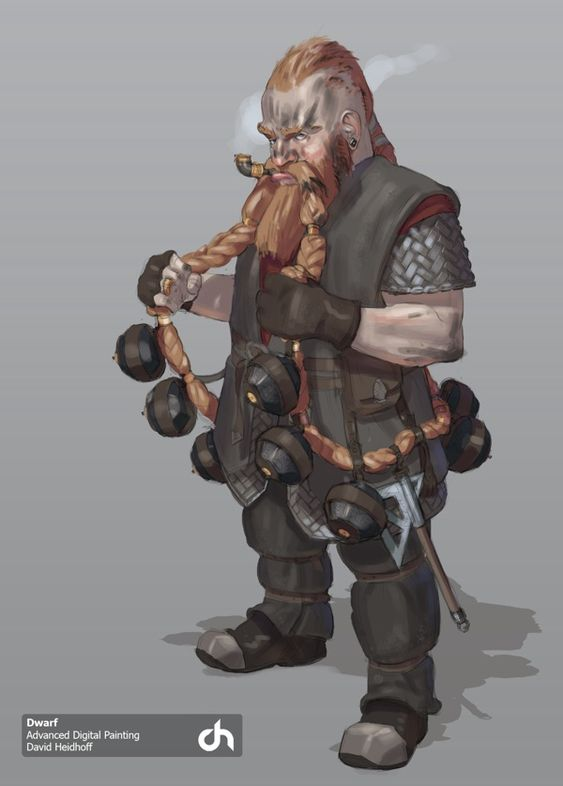
\includegraphics[width=0.49\textwidth]{alchimiste 1}
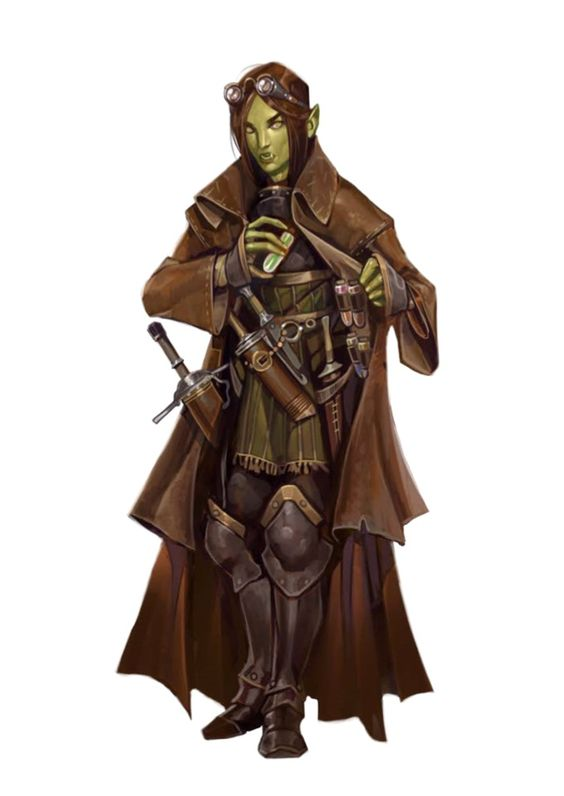
\includegraphics[width=0.49\textwidth]{alchimiste 2}
\subsection{Barbares}
Les barbares combattent avec férocité, une rage de vaincre qui leur permet de se dépasser toujours plus, et de vaincre leurs ennemis. Ce n'est pas sans douleur, mais c'est efficace.

Ce sont des combattants légers et mobiles, certains s'identifient à un totem animal, d'autres purement par leur rage.

Leur rôle dans un groupe d'aventurier est celui de première ligne : ils frappent fort, et peuvent encaisser beaucoup de coups avant de tomber.

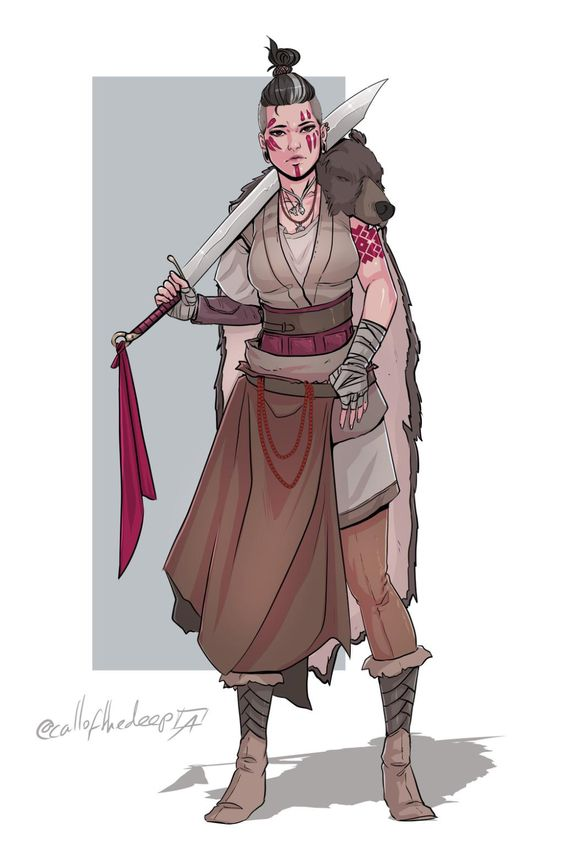
\includegraphics[width=0.49\textwidth]{barbare 1}
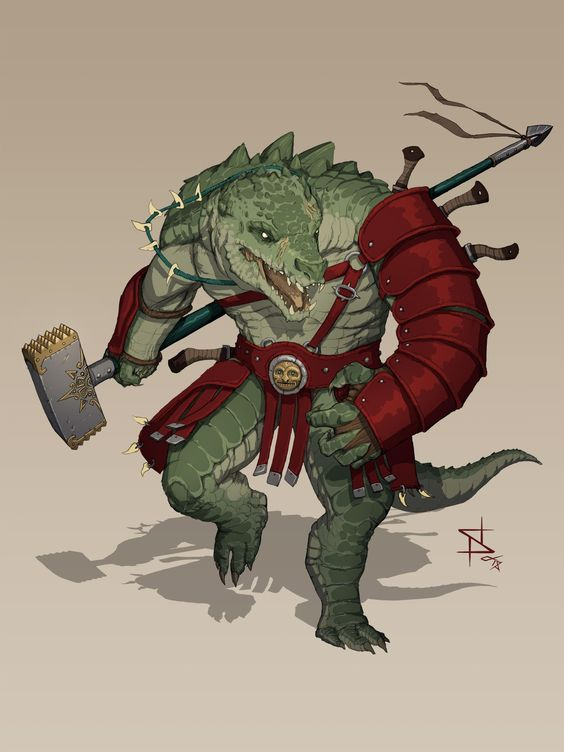
\includegraphics[width=0.49\textwidth]{barbare 2}
\subsection{Bardes}
Les bardes et artistes sont présents dans toutes les cultures. Ils fascinent les foules par leurs récits, chansons ou danses. 

La différence entre un barde et un autre artiste réside dans la magie que les premiers peuvent infuser dans leurs œuvres, leur permettant de contrôler les esprits, ou de déclencher des illusions.

En tant qu'aventuriers, ils sont le plus souvent des soutiens, encourageant leurs camarades à sans cesse accomplir des exploits, mais aussi à lancer leurs sortilèges sur leurs ennemis. Certains peuvent aussi participer plus directement au combat, souvent avec des armes légères. Ils peuvent alors servir de combattants mobiles.

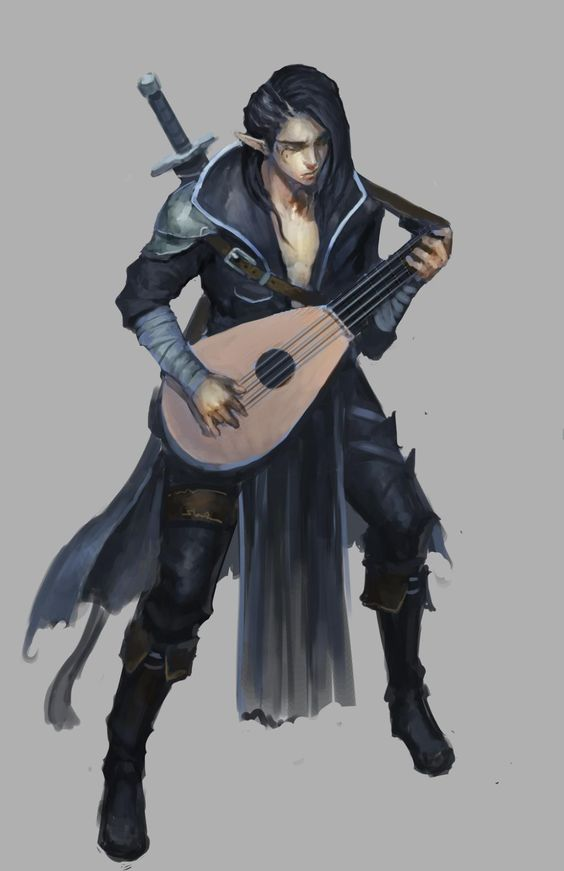
\includegraphics[width=0.49\textwidth]{barde 1}
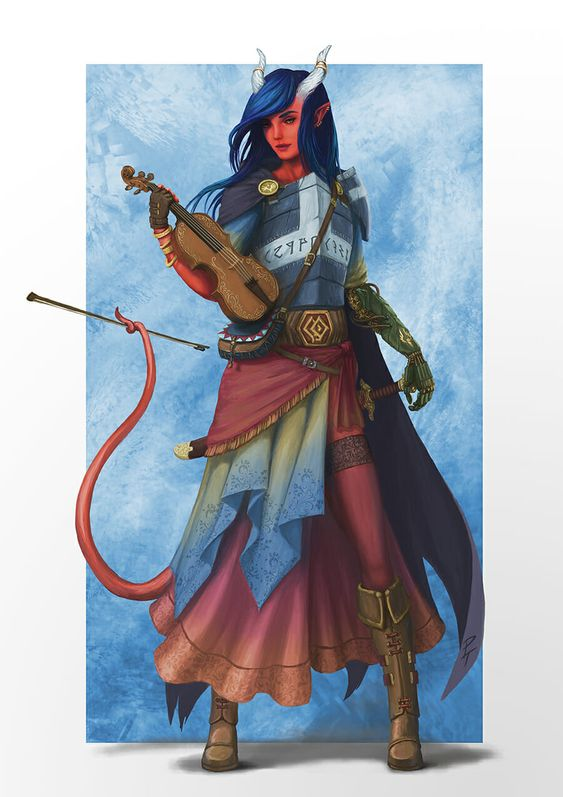
\includegraphics[width=0.49\textwidth]{barde 2}
\subsection{Champions}
Le champion a juré de défendre la cause d'une religion ou philosophie de vie, par les armes si nécessaire. A ses compétences martiales, il peut ajouter sa foi.

Sur le terrain, la plupart sont des combattants lourds, bien protégés pour mieux contre-attaquer. Et malheur à ceux qui servent une cause opposée à la leur.

A l'aventure, ils servent de première ligne, protégeant le reste du groupe des coups, tout en frappant l'ennemi de leur juste colère.

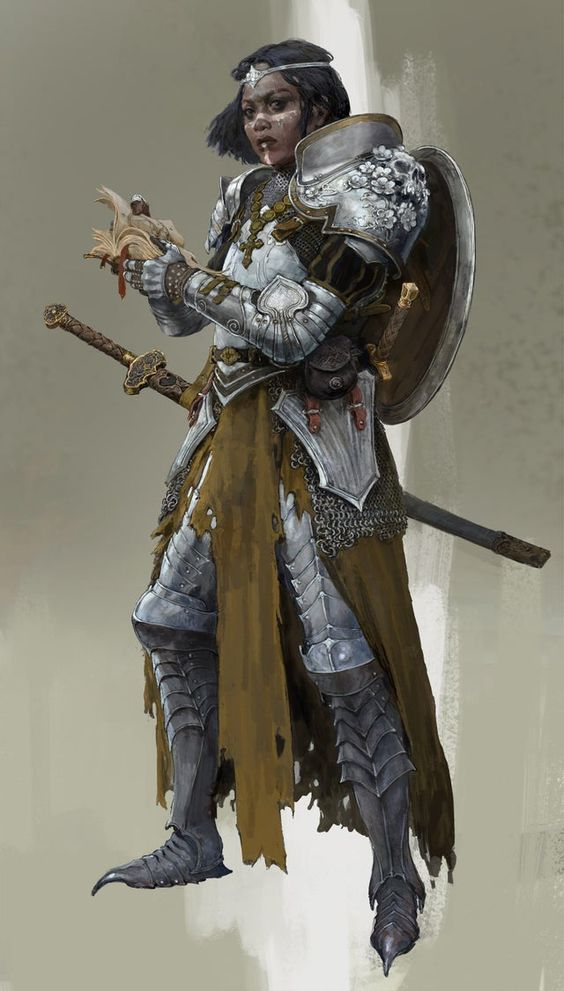
\includegraphics[width=0.49\textwidth]{paladin 1}
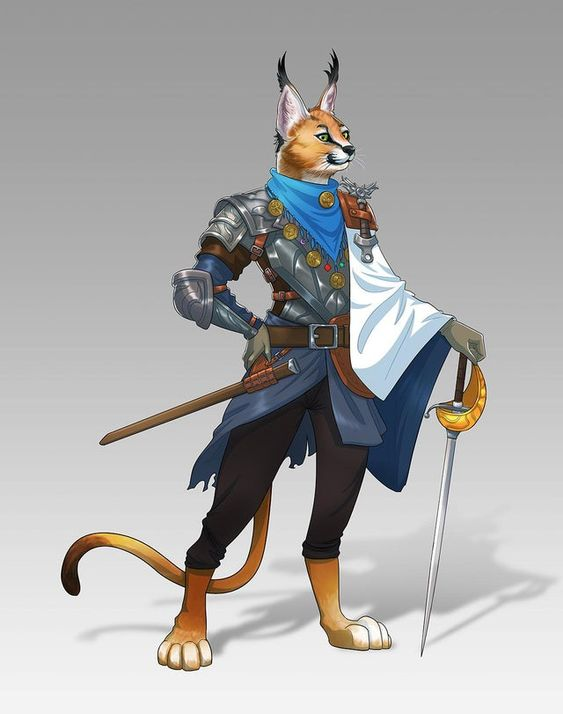
\includegraphics[width=0.49\textwidth]{paladin 2}
\subsection{Clercs}
Les clercs sont les plus fervents serviteurs des divinités de \nomorigine. Ils tirent leurs pouvoirs de leurs prières, et peuvent les perdre si ils déplaisent à cette divinité.

Il en existe autant de type que de divinités, voire plus, les églises n'étant pas toujours monolithiques dans leurs croyances et organisations.

Dans un groupe d'aventuriers, ils agissent en soutien : bénir leurs alliés et maudire leurs ennemis autant que possible, et parfois, mettre la main à la pâte pour frapper directement l'ennemi.

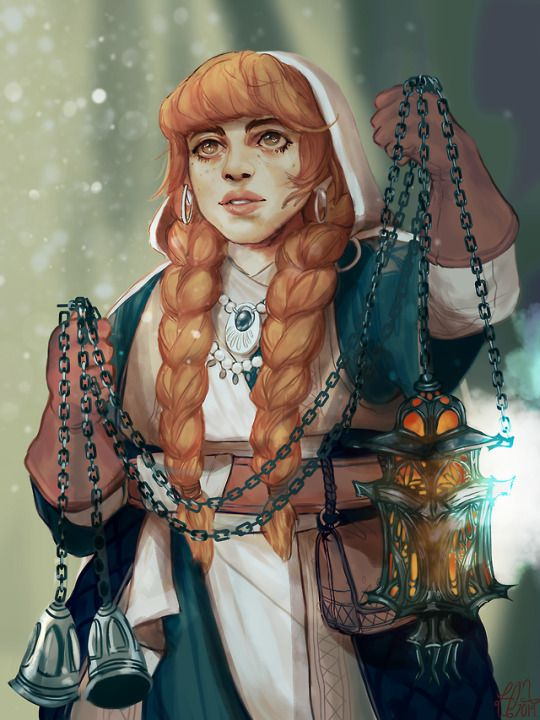
\includegraphics[width=0.49\textwidth]{clerc 1}
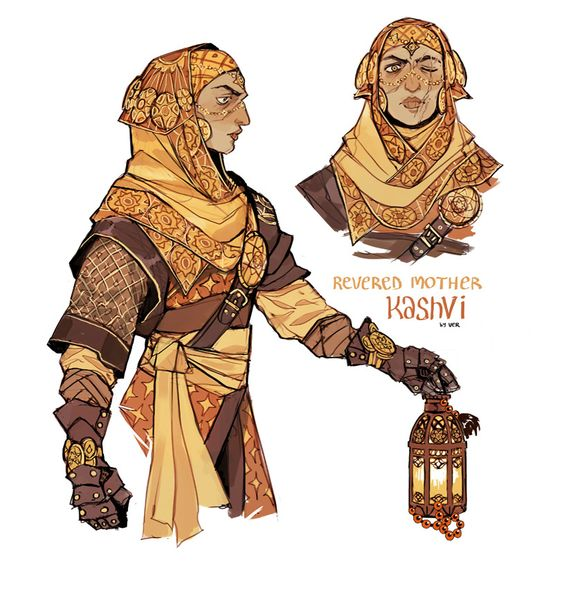
\includegraphics[width=0.49\textwidth]{clerc 2}
\subsection{Druides}
Les druides ont une profonde connexion avec la nature, au point de pouvoir lancer des sorts primaux. On les trouve le plus souvent dans les étendues sauvages, loin de la civilisation qu'ils n'apprécient guère.

Certains sont aussi sauvages que les animaux dont ils s'entourent, d'autres peuvent se rapprocher de prêtres de la nature, sans passer par l'intermédiaire d'une divinité.

A l'aventure, ils sont un soutien magique certains, ou une créature sauvage chassant ses proies, le plus souvent un peu des deux. Ils préfèrent les aventures dans les terres sauvages, qu'ils connaissent mieux que quiconque.

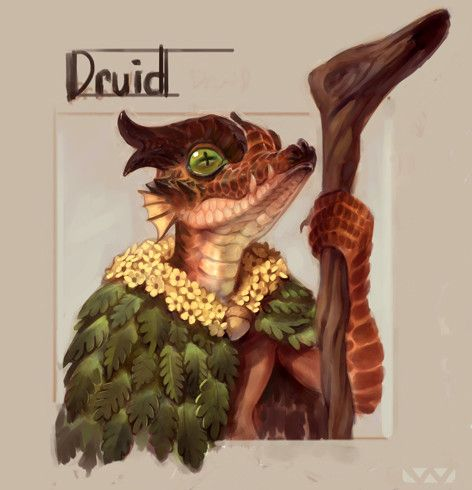
\includegraphics[width=0.49\textwidth]{druide 1}
\includegraphics[width=0.49\textwidth]{druide 2}
\subsection{Guerriers}
Les combattants experts existent dans toutes les cultures : dédiés à l'art de la guerre, ils sont bien au-delà du simple soldat.

Suivant leurs armes et armures de prédilections, ils peuvent prendre de nombreuses apparence : du tireur embusqué, au combattant en armure lourde, en passant par un duelliste de talent.

En tant qu'aventuriers, ils servent soit de première ligne, soit de tireurs, dans tout les cas, utilisant leur grande maîtrise des armes pour infliger mort et destruction.

\includegraphics[width=0.49\textwidth]{guerrier 1}
\includegraphics[width=0.49\textwidth]{guerrier 2}
\subsection{Investigateur}
L'investigateur n'est pas issue d'une ancienne tradition, c'est une science moderne. Ils se posent (et posent) constamment des questions sur leur environnement pour le comprendre, et résoudre les problèmes face à eux. Bon nombre d'entre eux viennent au départ des gardes des grandes villes.

Ils étudient soigneusement les problèmes afin de proposer des solutions efficaces. certains favorisent l'emploi de l'alchimie, d'autre de la médecine, d'autres encore sont des interrogateurs experts, enfin, certains analysent simplement très vite leur environnement.

A l'aventure, ils privilégient souvent les phases d'enquête, mais peuvent aussi identifier les points faibles des adversaires, ou utiliser leur tête pour faire tomber leur cible.

\includegraphics[width=0.49\textwidth]{investigateur 1}
\includegraphics[width=0.49\textwidth]{investigateur 2}
\subsection{Moines}
Les moines viennent de traditions différentes partageant un point commun : le perfectionnement physique, et en particulier la maîtrise des arts martiaux simples, permet de s'améliorer en tant que personne. Souvent issus de monastères ou d'écoles isolées, ils maîtrisent leur corps à la perfection.

Différentes écoles impliquent différents styles : certains favorisent la maîtrise de leurs corps pour accomplir des exploits quasi-surhumains, d'autres privilégient l'étude de styles de combat aussi gracieux que redoutables.

En tant qu'aventuriers, ils ont un rôle de cogneurs : il ne s'agit pas pour eux de prendre des coups, mais bien d'en donner.

\includegraphics[width=0.49\textwidth]{moine 1}
\includegraphics[width=0.49\textwidth]{moine 2}
\subsection{Oracles}
Les oracles tiennent leur pouvoir du divin, mais en paient lourdement le prix. Ils ne servent pas les dieux directement, mais doivent faire face à une malédiction qui les ronge.

Ce sont des lanceurs de sorts divins, testant très souvent les limites que leur impose leur malédiction. Suivant la façon dont leur révélation s'est manifesté, leurs capacités peuvent être très variées.

Dans un groupe d'aventuriers, ils servent fréquemment de soutien, avec leur arsenal de sorts divins, même si certains privilégient d'autres rôles (cogneurs ou combattants).

\includegraphics[width=0.49\textwidth]{oracle 1}
\includegraphics[width=0.49\textwidth]{oracle 2}
\subsection{Rangers}
Les rangers sont des éclaireurs, des trappeurs ou encore des chasseurs, distingués de leurs pairs par leur expérience ou un lien avec la nature. 

Certains se battent aux cotés d'un compagnon animal, d'autre privilégient le maniement des armes à distance. Enfin,certains manient deux armes avec un grand talent.

Dans un groupe d'aventuriers, ils servent souvent d'éclaireurs, en particulier en extérieur, et sinon, sont des cogneurs, infligeant de lourds dégâts à l'ennemi qu'ils chassent.

\includegraphics[width=0.49\textwidth]{ranger 1}
\includegraphics[width=0.49\textwidth]{ranger 2}
\subsection{Roublards}
Des brutes, des voleurs, des nobles ou encore des assassins. Leur point commun est de privilégier le travail dans l'ombre pour accomplir leurs objectifs : vols, intrigues et coups dans le dos sont leurs outils.

Certains sont de grands charmeurs, capables de berner leurs interlocuteurs, d'autres sont des combattants doués, comptant sur de nombreuses feintes pour déséquilibrer le combat en leur faveur.

A l'aventure, ils sont une sorte de joker hors combat, avec de nombreuses compétences et contacts. En combat, ils essaient de se faufiler pour poignarder l'ennemi dans le dos, ou d'utiliser des tactiques plus fourbes les unes que les autres pour triompher.

\includegraphics[width=0.49\textwidth]{roublard 1}
\includegraphics[width=0.49\textwidth]{roublard 2}
\subsection{Ensorceleurs}
Les ensorceleurs sont nés avec des talents magiques. Ils n'ont pas eu d'efforts à faire pour les développer ou les maîtriser, et souvent, on peut remonter ces pouvoirs à une influence magique sur leur famille : peut-être un ancien pacte, ou un lien plus direct avec une entité magique puissante.

Suivant leur lignage, les ensorceleurs profitent donc de pouvoirs variés : draconiques, primaux, ou encore infernaux. Contrairement aux mages,ils n'ont pas besoin de préparer leurs sorts, et peuvent donc plus facilement improviser. La contrepartie est une moins grande variété dans leurs choix de sorts.

Dans un groupe d'aventuriers, ils prennent le même rôle qu'un mage, capables de réagir plus rapidement à des circonstances changeante. Ils bombardent l'ennemi de sorts de contrôle ou de dégâts, suivant leur lignage.

\includegraphics[width=0.49\textwidth]{ensorceleur 1}
\includegraphics[width=0.49\textwidth]{ensorceleur 2}
\subsection{Bretteurs}
Les bretteurs sont des combattants avec comme point commun d'avoir une extrême confiance en leurs capacités et leur chance. Pour eux, le combat est une forme d'arts, presque une danse.

Ce sont des combattants légers, préférant éviter les coups, et riposter aussi vivement que possible. Leur confiance en eux leur permet également de  se distinguer : certains vont se vanter pour agacer l'adversaire, d'autres vont privilégier un style très acrobatique, certains seront d'excellent techniciens de leur lame, d'autres enfin vont danser sur le champ de bataille, passant presque délicatement d'un adversaire à l'autre.

Dans un groupe d'aventuriers, ils servent le plus souvent à infliger des dégâts à l'ennemi : de nombreux petits coups précis, mais dévastateurs sur le long terme.

\includegraphics[width=0.49\textwidth]{bretteru 1}
\includegraphics[width=0.49\textwidth]{bretteur 2}
\subsection{Sorciers}
Les sorciers tirent leurs pouvoirs d'un sombre pacte avec une entité plus ou moins connue. Ce pacte se manifeste sous la forme d'un familier envoyé par cette entité.

Les sorciers privilégient malédictions et bénédictions pour accompagner leurs sortilèges, leur rôle exact dépendant beaucoup de la nature de l'entité qui leur a confié ces pouvoirs.

A l'aventure, ils remplissent le rôle d'un mage : régler les problèmes par l'application de sortilèges. Ils y ajoutent fréquemment leurs malédictions, pour palier à une moins grande puissance magique.

\includegraphics[width=0.49\textwidth]{sorcier 1}
\includegraphics[width=0.49\textwidth]{sorcier 2}
\subsection{Mages}
Les mages ont appris leurs talents arcaniques par de longues études et un travail constant. De fait, ils maîtrisent un large éventail de sorts pour de nombreuses situations.

Ils divisent la magie en huit écoles de sorts, que sont l'illusion, la nécromancie, l'évocation (création d'éléments le plus souvent), l'invocation (appel de créatures), l'abjuration (briser d'autres sortilèges), la divination, l'enchantement (s'en prendre aux esprits des autres) et la transmutation (changer la matière). En plus de ces huit spécialités potentielles, il est possible de rester le plus généraliste possible.

Dans un groupe, ils ont un rôle de contrôle, modifiant le champ de bataille en fonction de leur volonté : sorts de vol, boules de feu, murs de pierres, mais aussi vision à distance, antimagie ou encore relever les morts font parti de l'arsenal du mage.

\includegraphics[width=0.49\textwidth]{mage 1}
\includegraphics[width=0.49\textwidth]{mage 2}
\end{document}